\chapter{ComBiNet: Visual Query and Comparison of Bipartite Dynamic Multivariate Networks with Roles}\label{ch:combinet}
\minitoc

\newcommand{\combinet}{ComBiNet\xspace}

In the previous chapter \autoref{ch:hsna-process-and-network-modeling}, I showed that \modelplural allow to model well historical documents, with \emph{traceability}, \emph{document reality}, and \emph{simplicity} properties.
However, no visual tools currently exist to specifically explore and manipulate this type of data.
In this chapter, I propose a \va interface aimed at exploring historical documents modeled as \modelplural, for historians to be able to reflect on their data and encoding and to follow in depth-analysis.
I answer \textbf{Q2} by analyzing tasks and questions historians have on their data and providing interaction mechanisms that would allow them to apply specific views and extraction, find errors and reflect on the annotations, and answer their high-level historical question through visual queries and comparison.

\paperbox{This chapter is an updated version of an article currently submitted to the journal Computer Graphics Forum (fast track), and a poster presented at the conference EuroVis 2022 \cite{pisterVisualQueriesBipartite2022}. It was a joint work with my advisors Christophe Prieur and Jean-Daniel Fekete. I did the development of the interface and led the discussions, evaluation, and writing of the paper.}

\section{Context}

Social scientists such as historians aim at characterizing the structure and dynamics of social groups of interest, in a region and period of time they focus on\cite{tilly1984retrieving}.
Their work essentially relies on documents---such as marriage acts, census records, surveys, and business contracts---to gather information about the life of important actors that they explore in-depth, or to draw conclusions on social aspects of groups in the society of that period and place.
Instead of drawing conclusions from their gathered knowledge and interpretations of the documents, a more systematic approach consists in constructing a social network from the documents and following a network analysis approach~\cite{wetherellHistoricalSocialNetwork1998}.
For this, they need to encode their documents to extract the persons and any other useful information in the text and transfer it into a structured file or a database.
Social scientists can then explore, validate, or refute their hypotheses by visualizing and analyzing the network structure and the connectivity patterns between the entities of the resulting network.

Currently, social scientists often model their datasets as simple networks where the nodes are the persons mentioned in the documents (see \autoref{ch:hsna-process-and-network-modeling}).
Usually, Two persons are then connected together in the network when they appear in shared documents.
This representation is easy to visualize and analyze but simplifies and distorts the information by hiding the documents that witness the relationships between the persons.
Thus, another approach consists in modeling the data as bipartite networks, where both the documents and the persons are represented as nodes and are connected together when a document mentions a given person~\cite{grandjeanAnalisiVisualizzazioniReti2017, rossiExplorationLargeDatabase2014, shafieHypergraphRepresentationsStudy2017}.

In addition, historical documents include time and geospatial information corresponding to the date and location of the events they refer to, and potentially additional information on the mentioned individuals such as their gender, profession, and date of birth.
These are often essential to understanding underlying social phenomena, as time, space, and classical social categories play an important role in sociological structures and dynamics\cite{lemercier12FormalNetwork2015}.
For these reasons, as we discussed in \autoref{ch:hsna-process-and-network-modeling}, historical sources and the underlying social events they refer to can be modeled well by \emph{bipartite} with \emph{roles},  \emph{multivariate} \emph{dynamic} networks. \emph{Bipartite} means that both persons and documents (or events, that are often witnessed by physical documents) are modeled as typed nodes. \emph{Multivariate} means that the nodes and links can carry additional attributes. \emph{Dynamic} means that time is a mandatory attribute of documents.
Furthermore, a link created between a person's node and a document's node (when the person is mentioned in the document), has an associated link type that models the \emph{role} of the person in the document/event.
Additionally, documents can optionally carry a geographical location.
This model unifies several social network models and allows the representation of historical documents with simplicity, traceability, and document reality, \ie the relationships appear as they are mentioned in the documents without distortions implied by projections\cite{cristofoliAuxSourcesGrands2008}.

More complicated models exist such as knowledge graphs\cite{opitzInductionLargeScaleKnowledge2018}, which are very expressive but hard to manipulate, especially for social scientists.
In contrast, most visual and analytics tools widely used by social scientists such as Gephi~\cite{Gephi} and NodeXL~\cite{NodeXL} enforce too simplistic network models and only provide limited interactions for exploring the network data, even if they provide the computation of several network measures.
This results in many social historians ending their analysis by plotting the network using a node-link diagram---which is hard to read with dense networks---, and identifying the most important actors with the help of centrality measures\cite{lemercierQuantitativeMethodsHumanities2019}.
Lemercier \& al describe this phenomenon the following: ``Network graphs of the “spaghetti monster” variety are a case in point. Often, in historical papers, they are used to show that a network is dense (and that the author has mastered the new technology). The narrative then comments on the individuals identified as central in the network. This approach can indeed be quite interesting, but it is hardly the only possible use for network analysis.\cite{lemercierQuantitativeMethodsHumanities2019}''.
\va tools guiding social scientists towards more complex exploration with the help of interaction mechanisms are therefore needed.
% Contrary to the early taxonomy of tasks on graphs~\cite{lee:hal-00851754}, with the data model we use, it becomes impossible to characterize a finite set of simple tasks to support, along with their associated visual representations and interactions techniques.

In this chapter, I present a \va system to explore and analyze Bipartite Multivariate Dynamic Social Networks, with the aim of supporting more complex historical analysis based on easy-to-use interactions, but also potential data correction.
I elaborated the tool based on four collaborations with social scientist colleagues.
I first collected important questions they each had on their data and transcribed them from a network analysis perspective.
The majority of the questions raised consisted in either finding specific patterns in the network---corresponding to specific groups or individuals exhibiting intriguing behaviors ---or in comparing several subsets of the network, in terms of network measures, attribute distributions, and their overlaps.

% In this paper, we thus present a visual analytic system to explore and analyze Bipartite Multivariate Dynamic Social Networks. Based on the needs and questions of our collaborators,
I hence focus on three high-level tasks: exploration, queries, and comparison of this type of network.
Users can explore the data using two layouts: a node-link bipartite view showing the sociological structure of the network, and a map layout based on the geolocation of documents.
I designed and implemented a new visual graph query system that allows us to build both topological and attribute constraints, based respectively on a node-link interactive representation, and dynamic widgets.
By easy-to-create queries, social historians are able to 1) detect erroneous patterns and reflect on their encoding process and 2) find relevant patterns which can answer their historical questions.
For this, I rely on the Neo4j graph database~\cite{neo4j} and its query language \emph{Cypher}.
Most visualization systems offer dynamic queries to hide the complexity of query languages.
However, using a rich data model, some queries are easier to refine using scripting than dynamic queries.
I implemented dynamic queries that also show the translated Cypher queries, and inversely, can translate textual queries into visual queries.
With that interface, social scientists can start building their queries with simple widgets and, if needed, complement them by editing the query, alone or with the help of power users.
Furthermore, they can export their query, the associated results, and its history at any point to share it with someone else or to start an analysis session from a previous result.
\name also implements subgraph comparison techniques, allowing the comparison of networks, network-related measures, and attribute distributions between the entities returned by the queries.
% In this first version of \name, we focused on the power of queries and comparisons and not usability so most of the explorations have been done by one of the authors or close to.
I validate the query and comparison system with a formative usability study and I demonstrate \name can be used to answer sociological questions by describing in depth several real-world use cases.

% 1) a succession of attribute and topological queries that are usually applied sequentially, from the simplest to the more complex, % which can be done with a graph database system and associated query language;
% \item The comparison of several query resulting subgraphs, in terms of connectivity metrics or attribute distributions
% and 2) the comparison of networks, measures, and attribute distributions, either between the entire network and the results of a query or between two separate query results.
% Several sophisticated tools exist to explore and analyze rich social networks, such as Gephi~\cite{Gephi}, NodeXL~\cite{NodeXL}, Jigsaw~\cite{Jigsaw}, or VERTIGo~\cite{cuenca_vertigo_2021}. However, these tools often enforce a data model which are often either too simple
% except for Jigsaw, they provide too limited interactions to query and explore richly encoded data.

% Social Science use node link diagram
% There are now bipartite approaches
% Historical sources use time, attributes, locations. there should be more of these
% Need tools to explore these specific kind of dataset
% Query and comparison to answer historical and sociological questions

After the related work section, I describe our design process in \autoref{sec:combinet-tasks}, present the system \name in \autoref{sec:combinet-system} with the design of the visual query and comparison features, and present four use cases demonstrating the utility of the system in \autoref{sec:combinet-usecases} showing it can be used to explore complex historical data and allowing historians to answer several of their questions using queries and comparisons.
I finish with the results of the formative usability study in \autoref{sec:combinet-usability}.
%Our contributions are:
%\begin{itemize}
%% \item The description, motivations, and benefits of our unified data model: \emph{bipartite} with \emph{roles}, \emph{multivariate} and \emph{dynamic}, for the visual exploration and analysis of social networks;
%% \item The design and implementation of a bipartite graph visualization and map layout specific to social scientist needs.
%    \item The design and implementation of a graph query system, synchronizing the visual representation of the query and the associated script;
%    \item The design and implementation of visualization and interaction techniques aimed at comparing subgraphs, in terms of topology, attributes, time, and geographical location.
%    \item A usability study and three real-world use cases demonstrate the utility of the system to answer socio-historical questions.
%\end{itemize}



\section{Related Work}\label{sec:combinet:related-work}

As I already discussed the related work on network modeling and social network visualization in \autoref{ch:related-work} I only discuss in this section the related work on graphlet analysis, visual graph querying, visual graph comparison, and provenance.

\subsection{Graphlet Analysis}

One of the inspirations for this project came after participating in the 2020 VAST challenge\footnote{This is a challenge organized in the context of the IEEE Visual Analytics Science and Technology (VAST) conference. The challenge consisted of a series of analytical questions united under an overarching cyber threat scenario. We participated in the Mini-Challenge 1 which asked participants to identify a group of people that accidentally caused an internet outage. To identify this group, we were given a network profile and a large multi-variate social network to search in.} where our team used graphlets to measure similarity between several networks~\cite{tovanichVAST2020Contest2021}.

Graphlets are small connected induced, non-isomorphic subgraphs composing any network (see \autoref{subsec:methods-and-measures} for more details).
They were first introduced by Milo et al.~\cite{miloNetworkMotifsSimple2002} to explore the structural differences between biological networks, but they are now used in several disciplines involving networks such as sociology\cite{charbeyStarsHolesPaths2019}.

One of the aims of the VAST 2020 challenge was to compare several multivariate networks.
However, by using graphlets we realized that 1) it was not very efficient to compare several networks in contrast to other measures, and 2) the interpretation of all graphlets patterns that are found in a network is complicated given the fact that one specific pattern can have various interpretations given the nodes involved and their positions in the network~\cite{ingramNetworkMotifsStructure2006}.
This is especially true that the number of potential graphlets grows exponentially as we increase the number of nodes considered (there are 6 graphlets of size 4 and 21 graphlets of size 5 for example) and if we add complexity to the network model, for example by using directed links or node and link types~\cite{ribeiroDiscoveringColoredNetwork2014}.

Instead of counting every graphlet occurrence and interpreting them with sociological meanings, it appeared more efficient to let social scientists find specific patterns to answer questions they already ask themselves on the data.


\subsection{Visual Graph Querying}


% Guess~\cite{adar_guess_2006} has been designed to provide a dual view of networks, one from a scripting language (a variation of Python) coupled with a visual representation of the network. However, it still relies on scripting to search and manipulate the network, contrary to modern visualization systems using dynamic queries~\cite{DynamicQueries}.

Graph pattern matching is an important task in \sna, which consists in finding a subgraph of interest in a larger graph\cite{fanGraphPatternMatching2012}.

Several scripting languages, such as R~\cite{Rstat} and Python~\cite{Python}, have been extended to support the exploration of social networks using specialized libraries such as igraph~\cite{igraph} and NetworkX~\cite{NetworkX}, and provide functions for graph pattern matching.
However, social scientists are often challenged to use scripting languages and programming, as they often do not have formal training in such technologies.

Graph databases allow to storage and manipulation of network data with the use of query languages, such as the Cypher language for Neo4j\cite{neo4j}.
%Constructing and querying a pattern from a graph requires knowledge of graph databases and query languages.
To lower the complexity barrier of their usage, several visual graph query systems have been developed to allow analysts to rapidly build and refine their queries visually.
Some systems hide the scripting language such as GRAPHITE~\cite{chauGRAPHITEVisualQuery2008} and VERTIGo~\cite{cuencaVERTIGoVisualPlatform2021} that allow specifying a graph query as a node-link diagram that the user creates interactively.
Shadoan and Weaver~\cite{shadoanVisualAnalysisHigherOrder2013} use a similar concept with hypergraphs to filter multidimensional data.
Other systems, such as VIGOR~\cite{pientaVIGORInteractiveVisual2018} only visualize the query after it has been written by the user with a scripting language and does not allow direct interaction of the visual representation of the query.
All these visual query systems are limited to topological queries with constraints on the vertex and edge types and do not allow to make constraints on other dimensions such as attributes and time associated with vertices and edges.

\iffalse
\subsection{Tasks Taxonomies}

Lee et al.~\cite{lee:hal-00851754} have introduced a taxonomy of tasks related to general graphs.
It relies on the taxonomy of low-level activities by Amar et al.~\cite{Amar05}, and extends it by considering different types of tasks: topology-based, attribute-based, browsing, and overview. These tasks can be applied to different kinds of graph-specific objects: nodes, links, paths, and various kinds of groups.
They also mention higher-level tasks but not time.

This taxonomy has been extended for dynamic networks by Bach et al.~\cite{bach:hal-00906597} and Ahn et al.~\cite{Ahn14}, using a similar method of applying the low-level taxonomy of Amar et al.\ to all the graph objects plus time. The method reaches its limit here since the number of tasks is proportional to the Cartesian product of the objects considered and time, and becomes too large to be fully discussed.
In parallel, Adrienko \& Andrienko~\cite{andrienko2006exploratory}
Kerracher et al.~\cite{Kerracher15} summarize these taxonomies \jdf{Revise the Andrienko' taxonomy for our bipartite networks.}

None of these taxonomies mention ``comparison'' as a primary task, maybe because, in their reference taxonomy of interaction techniques, Yi et al.~\cite{yiDeeperUnderstandingRole2007} write: ``we debated adding a \emph{Compare} category but ultimately
omitted it because we believe that Compare is a higher-level user goal or objective than the other user intents we identify''. Gleicher~\cite{Gleicher18, gleicherVisualComparisonInformation2011} develops an abstract framework to clarify the ``comparison'' task in visualization and argues for its importance.
We agree with Gleicher since several of the use cases reported by our social scientists' colleagues involve comparisons.
\fi

%\vspace{-2mm}
\subsection{Visual Graph Comparison}

Gleicher et al.~\cite{Gleicher18} propose a taxonomy of visual comparison designs for complex objects. They claim any visual comparison system can be classified into one (or a mix) of the three following categories: juxtaposition, superposition, or explicit design.
Yet, few visual systems support comparison tasks for social networks.

Andrews et al.~\cite{andrewsVisualGraphComparison2009} describe a technique to compare several networks, using a combination of juxtaposition and superposition techniques.
The two candidate networks are shown side by side, along with a third view composed of a fusion network highlighting both the shared nodes along with the non-shared nodes with different colors.
%
Freire et al~\cite{ManyNets} describe the ManyNets system to compare many networks by using a table where each describes one graph and each column shows graph measures in terms of small visualizations, from simple bars to distributions, allowing the comparison of a large number of graphs. However, ManyNets does not visualize the networks per se (no layout shown), and do not take into account attributes, node types, or time.
%
Hascoët and Dragicevic~\cite{HascoetD12} describe a system to match and compare graphs using superposition, focusing on the topology, not taking into account attributes or time.
Tovanich et al.\cite{tovanichVAST2020Contest2021} propose a visual analytics tool to compare multivariate, sometimes bipartite, dynamic networks and find common structures.
However, the tool does not handle roles and is designed for the specific task of matching a subgraph into a larger network.

\subsection{Provenance}

Provenance in the context of Visual Analytics consists in the logging of the sequence of actions of users on an interactive visualization system during analysis sessions.
Collecting provenance information has proven to benefit users by providing them action recovery (undo) plus collaborative and reproducibility capabilities~\cite{raganCharacterizingProvenanceVisualization2016}.
For example, the VisTrails system allows users to reproduce their visual analyses by providing an executable history graph of their actions,~\cite{callahanVisTrailsVisualizationMeets2006} while GraphTrail provides provenance tools to ease collaborative analysis~\cite{dunneGraphTrailAnalyzingLarge2012}.
Provenance can also be beneficial for visualization designers and researchers, as it gives them a tool to understand users' behaviors~\cite{battleCharacterizingExploratoryVisual2019, borsProvenanceTaskAbstraction2019}
and evaluate/improve visualization systems~\cite{renCharticulatorInteractiveConstruction2019}.
All the reasons and concrete implementations of provenance are discussed in depth in Xu's survey~\cite{xuSurveyAnalysisUser2020}.

\section{Task Analysis and Design Process}\label{sec:combinet-tasks}

I designed the \name tool in collaboration with social historians who wanted to follow a network analysis on their historical semi-structured documents, that are well modeled by \modelplural.
I first collected questions they had about their data and what they wanted to see in a visual interface.
By analyzing the questions we leveraged tasks and requirements that I used to design and implement the interface, with continuous feedback from our collaborators.
%We designed the interface from the requirements with continuous discussions with our collaborators.
%We showed them visual prototypes during the development phase to get feedback iteratively.

\subsection{Use Cases}

We elaborated this interface from the collaborations with historians I described in \autoref{subsec:hsna-examples}.
These collaborations involved regular meetings and multiple discussions over three years.
All these datasets are textual corpora constituted of historical documents mentioning people with complex relationships, which are well modeled with \modelplural.
We give more details about the datasets of these collaborations in this section, along with our collaborators' main questions with the associated network queries to answer them.
The full answers involve visualizations of the query results and attribute summaries that I describe in the next section.
%We list the most important questions our collaborators shared with us on their respective datasets.
We categorized the questions according to four dimensions: global (G)/local (L) (do they want to categorize a group of nodes or retrieve specific persons/documents), if the question can be answered using the topology (T), and/or the attributes (A), and finally if a comparison (C) using several filters is needed or not (N).

\begin{enumerate}
    \item Analysis of the social dynamics from \textbf{construction contracts in Italy in the 18\ts{th} century (141 documents, 272 persons)~\cite{Cristofoli2018}.}
    The corpus is made of contracts (manuscript documents) for different types of constructions in the Piedmont area in Italy. People are mentioned in three different roles: \textit{Associates}, who participate in the construction; \textit{Guarantors}, who bring financial guarantees; and \textit{Approvers}, who vouch for the guarantors. Along with the time and location of the construction site, documents have a construction type (military, religious, and civil), work type (big work, small work, reparation, transportation, etc.), and material (wood, stone, metal). People also have an origin attribute (the place they come from), manually extracted from the original documents.
    \begin{footnotesize}
    \begin{description}
    \item[Question 1] Do approbators act as bridges compared to associates and guarantors? (G, T, C)
    \item[\myindent Query 1.1] Request all approbators occurrences
    \item[\myindent Query 1.2 ] Request all associates and guarantors occurrences
    \item[Question 2] Are there people mutually guarantors to each other in different contracts? (G, AT, N)
    \item[\myindent Query 2.1] Select pairs of people connected each to the two same document, with a guarantor role and any other role
    \item[Question 3] Who are the persons of the extended Zo family (G, AT, N)
    \item[\myindent Query 3.1] Request all the persons of the Zo family and their N+2 ego network
    \item[Question 4] Compare the Menafoglio and Zo families in terms of contracts and activities (G, AT, C)
    \item[\myindent Query 4.1] Request all the persons of the Menafoglio family and the documents that mention them
    \item[\myindent Query 4.2] Request all the persons of the Zo family and  the documents that mention them
    \item[Question 5] Who are the persons having the 3 roles? (G, AT, N)
    \item[\myindent Query 5.1] Select persons with associate, guarantor, and approbator roles in 3 different documents
    \item[Question 6] What are the differences between Torino and Torino surroundings, concerning the types of constructions and actors involved? (G, AT, C)
    \item[\myindent Query 6.1] Request all documents located in Torino, with the persons mentioned
    \item[\myindent Query 6.2] Request all documents located in the Torino area, with the persons mentioned
    \end{description}
    \end{footnotesize}

    \item Analysis of migrations from the \textbf{genealogy of a french family between the 17\ts{th}--20\ts{th} centuries (2053 events, 957 persons from a private source).}
    The corpus is made of family trees referring to several document/event types: birth and death certificates, marriage acts, military mobilization, and census report. The roles are different for each event type and consist of \textit{children, father, mother} for the birth events, \textit{deceased} for the death event, \textit{spouse} and \textit{witnesses} for the marriages, and \textit{family member}s for the census events.
    \begin{footnotesize}
    \begin{description}
    \item[Question 7] What is the trajectory of life for a given specific individual (birth, living, marriage, death) (L, A, N)
    \item[\myindent Query 7.1] Select one person and all her/his documents (to use the mentioned places)
    \item[Question 8] What is the trajectory of life for a family (L, A, N)
    \item[\myindent Query 8.1] Select birth certificates with the child, parents, and birthplace
    \item[Question 9] Where are located the main migrations, and at which time do they occur? (G, A, N)
    \item[\myindent Query 9.1] Select persons with a geolocated birth and death certificate
    \item[Question 10] Are there differences in volume and location between migrations in the 18\ts{th} and 19\ts{th} centuries? (G, A, C)
    \item[\myindent Query 10.1] Select persons with a geolocated birth and death certificate from the 18\ts{th} century
    \item[\myindent Query 10.2] Select persons with a geolocated birth and death certificate from the 19\ts{th} century
    \item[Question 11] In the Haute-Vienne and Cote d'Armor administrative areas, are there cycles in living places every 10/20 years? (G, A, N)
    \item[\myindent Query 11.1] Select persons with their census reports located in Cote d’Armor and Haute-Vienne
    \item[Question 12] In the 19\ts{th} century, was there an overall decrease in the social status and professions of persons in the dataset? (G, A, C)
    \item[\myindent Query 12.1] Select persons in the first half of the 19\ts{th} century with a profession mentioned
    \item[\myindent Query 12.2] Select persons in the second half of the 19\ts{th} century with a profession mentioned
    \end{description}
    \end{footnotesize}
%6659 PERSONS. 1381 MARRIAGE_ACTS.
    \item Analysis of migrations from Spain to Argentina through the \textbf{marriage acts at Buenos Aires in the 17--19\ts{th} centuries (1381 acts, 6659 persons)~\cite{moutoukiasBuenosAiresPort2016}.}
    The corpus is made of acts that mention the spouses and the witnesses of the wedding, which are the roles modeled by the links. The origin, date of birth, and parents' names are specified for both spouses.
    % These parenting relationships are important for our collaborator, but do not refer to the same event as the marriage. Thus, we create another event node referencing the birth event, with \textit{father, mother}, \textit{child} as roles and the associated birth year and location as node attributes.
    \begin{footnotesize}
    \begin{description}
    \item[Question 13] How are spouses and witnesses linked in their family network? (G, T, N)
    \item[\myindent Query 13.1] Select marriages with spouses and witnesses, where the spouse and witnesses have the same parents
    \item[\myindent Query 13.2] Select marriages with spouses and witnesses, where the spouse and witnesses have the same grandparents
    \item[Question 14] Who are the persons with 2 marriages with a long delay? (L, A, N)
    \item[\myindent Query 14.1] Select persons in 2 marriages as husband or wife. Put a constraint on the difference of time in the marriages
    \item[Question 15] Where are the persons marrying in Buenos Aires coming from? (G, A, N)
    \item[\myindent Query 15.1] Select persons with a birth certificate not located in Buenos Aires
    \end{description}
    \end{footnotesize}

    \item Socio-political analysis of \textbf{migration of ethnic Germans from communist Romania to West Germany in the 20th century (ongoing work)~\cite{diminescuMigrationEthnicGermans2020}.}
    The corpus is made of administrative forms that mention persons requesting to migrate, along with the persons they want to join, and the administrative persons of the ministry in charge of the forms (3 roles).
    The family members of the aspiring migrant are also mentioned in the forms, with their respective dates of birth.
     \begin{footnotesize}
    \begin{description}
    \item[Question 16] What members of their family do emigrants usually join? (G, AT, N)
    \item[\myindent Query 16.1] Select all migration documents with the emigrant and the person they are joining
    \item[Question 17] What price does the emigrant have to pay, given their socio-economic profiles? (G, A, C)
    \item[\myindent Query 17.1] Select people who are mentioned in a budget and a migration document
    \end{description}
    \end{footnotesize}
\end{enumerate}


\subsection{Tasks Analysis}

Most of the questions we collected from our collaborators could be answered by isolating a subgroup of entities and analyzing them in the context of the whole network, or by comparing two subgraphs, in terms of their entities, structure, and attribute distributions.
From discussions with our collaborators and the analysis of their questions on their data, we elaborated a list of requirements for the visual interface, split into three main parts: 1) Exploration of the data, 2) Queries, and 3) Comparisons.
The elaboration of the tasks was an iterative process, as we showed the interface to our collaborators several times in the development phase to get feedback.
The tasks are described here and summarized in \autoref{tab:tasks}:

\begin{enumerate}
    \item \textbf{Exploration of \model}. The visual interface must allow exploration of this specific type of network, using every aspect of the data, i.e.\ its topology (T1.1), node attributes  (T1.2), roles (T1.3), geolocation of the documents/events (T1.4) and time (T1.5).
    Common interactions such as selection and zooming are also needed for the exploration.
    \item \textbf{Applying filters}. To answer their questions, users need to be able to apply filters to the data, to isolate specific groups of entities having specific behaviors or characteristics. To answer the diversity of questions, they should be able to put constraints on every aspect of the data, i.e.\ the topology, the roles (T2.1), and the attributes (including time and geolocation) (T2.2).
    % As queries can be quite complex, we want users to be able to write their queries textually (T2.3).
    Access to provenance information can also help them in their query construction, by going to previous states and exploring different paths more easily (T2.3). Once they are satisfied with their query, they want to explore the results, usually in the context of the whole network (T2.4).
    \item \textbf{Comparison of several subgraphs.} Users should be able to compare several subgraphs isolated after applying filters, to see the similarities and differences between groups of entities of interest. The system should be able to easily see the common and shared entities of the two subgraphs (T3.1), their respective place in the network, their structural differences (T3.2), and their different attribute distributions (T3.3).
\end{enumerate}


\begin{table*}
    \center \scriptsize
    \begin{tabular}{|l|V{4cm}|l|V{2cm}|}
        \hline
        Main Tasks & Subtasks                                                       & Views    & Constraints \\ \hline
        \multirow{5}{*}{Bipartite Graph Exploration} &
        T1.1 Overview of the network &
        V1 &
%        \multirow{5}{*}{\begin{tabular}[c]{@{}l@{}}A node-link representation is expected.\\ The geolocation of events has to be done according to the historical period.\end{tabular}} \\ \cline{2-3}
        \multirow{5}{*}{\parbox{2cm}{A node-link representation is expected.\\ The geolocation of events has to be done according to the historical period.}} \\ \cline{2-3}
        & T1.2 Overview of nodes attribute values and distributions        & V1,V2,V4 &             \\ \cline{2-3}
        & T1.3 Show the persons' roles in the documents they appear in & V1       &             \\ \cline{2-3}
        & T1.4 Show the location of the different documents               & V2       &             \\ \cline{2-3}
        & T1.5 Show the time of the documents                            & V1,V2,V4 &             \\ \hline
        \multirow{5}{*}{Apply filters to isolate subgraphs} &
        T2.1 Filter on topological patterns &
        V6, V8 &
        \multirow{4}{*}{\parbox{2cm}{Constraints must be easy to set and visual.}} \\ \cline{2-3}
        & T2.2 Filter on attribute values                                & V7,V8       &             \\ \cline{2-3}
        & T2.3 Show the provenance of filters      & V9   &             \\ \cline{2-3}
        & T2.4 Show the subgroups alone or in the network's context & V1, V2 &             \\ \hline
        \multirow{3}{*}{Compare several subgroups} &
        T3.1 Show the shared and exclusive entities &
        V1/V2 &
        \multirow{3}{*}{} \\ \cline{2-3}
        & T3.2 Compare the node attribute distributions                  & V4       &             \\ \cline{2-3}
        & T3.3 Compare the subgraph measures                             & V3       &             \\ \hline
    \end{tabular}
    \caption{Tasks to support during exploration, according to our expert collaborators, are split into 3 main high-level tasks. }\label{tab:tasks}
\end{table*}


\section{The \name System}\label{sec:combinet-system}

\begin{figure}[!ht]
 \centering
    \begin{overpic}[width=\textwidth]{static/figures/ComBiNet/OriginalPaperFigures/CGF/teaser/v2/teaser}
    \put(30,17){\tiny Comparison}
    \put(6, 2){\circledColored{\small A}{blue}}
    \put(20, 2){\circledColored{\small B}{red}}

    \put(15, 26){\circled{\tiny V6}}
    \put(23, 16){\circled{\tiny V7}}
    \put(23, 8){\circled{\tiny V8}}
    \put(73, 21){\circled{\tiny V1}}
    \put(95, 21){\circled{\tiny V2}}
    \put(42, 18){\circled{\tiny V9}}
    \put(95, 2){\circled{\tiny V3}}
    \put(64, 10){\circled{\tiny V4}}
    \put(95, 10){\circled{\tiny V5}}
    \end{overpic}

    \caption{The \name system used to compare two subgroups of a social network of contracts from \protect\cite{Cristofoli2018}, extracted with dynamic visual queries. (A) and (B) show the two visual queries created by the user in the query panel using an interactive node-link diagram editor (V6), dynamic query widgets (V7), and the equivalent Cypher script (V8). The right part shows \name's global interface in \textit{comparison} mode: (V1) Network visualization panel, (V2) Map of the geolocalized nodes, (V3) Table of persons, (V4) Graph measures comparison, (V5) Attribute distribution plots, and (V9) Provenance tree. The two visual queries on the left, translated into Cypher queries below, select the ``Menafoglio'' family on the left, and the ``Zo'' family on the right, along with their construction contracts and close collaborators.
    }\label{fig:combinet-overall}
\end{figure}

\name is designed to visualize, explore, and analyze social networks encoded as \model.
Some other systems exist to explore bipartite social networks such as Jigsaw and Puck, but do not encode every aspect of historical documents historians are interested in.
\autoref{tab:combinet-VA-comparison} shows a comparison of their data model compared to \name.

\begin{table}[]
\centering
\resizebox{\textwidth}{!}{%
\begin{tabular}{|l|l|l|l|l|l|}
\hline
         & Bipartite & Node Attributes & Links Attributes & Dynamic & Geolocated \\ \hline
Jigsaw   & \cmark    & Only some       & \xmark           & \cmark  & \cmark     \\ \hline
Puck     & \cmark    & \xmark          & \xmark           & \cmark  & \xmark     \\ \hline
ComBiNet & \cmark    & \cmark          & Encode roles     & \cmark  & \cmark     \\ \hline
\end{tabular}%
}
    \caption{Comparison of the data model of several VA systems aimed at exploring bipartite social networks.
    }\label{tab:combinet-VA-comparison}
\end{table}


When started, \name dynamically collects the node types, roles, sub-types, and attributes when reading the network from the database. The interface is constituted of four main panels, split into different views as shown in\autoref{fig:combinet-overall}: the query and comparison panel (V6, V7, V8, and V9), the bipartite visualization panel (V1), the map visualization panel (V2), and the query results panel (V3, V4, V5).
I present in the following the different views, according to their visualization or query functions.
Comparison features are incorporated in the same views with different comparison mechanisms.


\subsection{Visualizations}

\name presents a social network with multiple visualizations and views highlighting different aspects of the data.
The views are linked when it makes sense so that interactions such as selection done on one propagate to other views.

\noindent\textbf{V1: Bipartite Node-Link View}
The bipartite node-link visualization panel shows the network using the DrL force layout from igraph~\cite{igraph} with overlap removal using D3~\cite{d3}.
Node-link representations are very common in social sciences~\cite{Gephi, mrvarAnalysisVisualizationLarge2016, NodeXL, cristofoliPrincipesUsagesDessins} and were a specific request from our collaborators.
In the context of our bipartite model, the persons are represented as circles and the documents/events as squares, while the roles are encoded as link colors.
A link models the mention of a person in a document.
This view provides an overview of the data by showing the structure of the network (T1.1) and the roles of the persons in their different documents (T1.2).
%Attribute values can be overlayed on the nodes using colors when users select an attribute. It allows detecting patterns relative to attributes, in the context of the topology of the network (T1.2, T1.4, T1.5). For example, \autoref{fig:combinet-time-selected} shows the construction dataset of \pascal where the user selected the \textit{year} attribute, coloring the documents nodes with their year in the node-link diagram (left).
The view also provides pan \& zoom and selection interactions for effective navigation.
Nodes' labels are displayed (name of person and ids of documents by default) on the canvas with an occlusion-free mechanism that hides nodes with a low degree when two or more nodes' labels overlap.


\noindent\textbf{V2: Map View}
The map visualization panel on the right shows an event-centric view, displaying only the geolocalized event nodes on a map.
By default, only event nodes are shown, but users can select a threshold to show links between nodes when they share at least a given number of persons in their mentions.
%The system can create links between event nodes that share persons with a user specified threshold.
% A link is created between two nodes when the two events share at least one person.
Persons are not directly shown in this view as they do not have a unique location.
This map view presents a transformation of the bipartite network, focused on the geospatial information that is very important to social scientists (T1.3).

As we collaborate with historians who study different periods, we cannot use modern map backgrounds such as the default one provided by OpenStreetMap or Google Maps since many features are anachronistic (\eg roads, administrative areas, borders). We, therefore, provide a map background with only these non-administrative features: elevation, lakes, rivers, and types of environment.
We also show the most important cities as most of them existed in the past and provide landmarks.
The map uses Natural Earth tiles and vector data~\cite{NaturalEarth}.

The map has the same interaction mechanisms as the bipartite node-link view.
The two views are also coordinated: selecting/hovering an event node in the graph view highlights it on the map and vice versa, while hovering a person node highlights all its corresponding documents on the map, rapidly showing the person's events' locations.
%The views are also linked to the entities tables: selecting a node highlights the corresponding row and pushes it at the top of the table.

\noindent\textbf{V3: Entities Tables}
All the persons and the documents of the loaded dataset are listed in two separate tables, showing the attributes of the entities (person or document).
This way, users can order the entities according to any attribute they want (T1.2).
The tables are linked to the visualizations, meaning that selecting a row highlights the respective entity in the visualizations and vice-versa.
Selecting a node hence highlights the corresponding row and pushes it to the top of the table.
Tables in social network visualization systems have been proven to be efficient and useful for social scientists when exploring their data~\cite{bezerianosGraphDiceSystemExploring2010} and are a feature that has been asked by our collaborators.
It allows them to link the visualization to the network entities more easily, and dive deeper into one entity's attribute values after selecting it in the network.
For example, if the visualization reveals an intriguing person connected to two distant components through two documents, the user can rapidly see the information of this person and documents on the tables, to see if this could be an error from the annotations or an interesting person he or she could investigate more in depth in the original sources.
It also makes ranking entities according to various criteria easier and more straightforward.
Finally, the tables are exportable in CSV, pdf, or directly in the clipboard, which was a request to our collaborators.



\noindent\textbf{V4: Graph Measures}
The Graph Measures view shows measures related to the network and gives insights into its structure to users (T1.1).
We report simple measures like the number of persons, documents, links, and components, and more sophisticated bipartite network measures asked by our users, that they can report for their analysis: the bipartite density, bipartite average clustering coefficient, and bipartite average redundancy\cite{latapyBasicNotionsAnalysis2008}.
These measures are updated in real time when filters and comparisons are applied.


\noindent\textbf{V5: Attributes View}
All the attributes in the network are shown as buttons in the bottom right of the interface, sorted by their associated node type (person, document, and ``All'' for both types).
They can be quickly visualized by hovering over the button, producing two effects: it colors all the nodes on the two views according to their attribute values, and it shows a plot of the distribution of the selected attribute. \autoref{fig:combinet-time-selected} shows the construction dataset of collaboration \pascal where the user selected the \textit{\_year} attribute, coloring the documents nodes with their year in the node-link diagram (left) and the map view (right), revealing for example that most construction occurring in 1714 occurred in Torino and Torino close surrounding.
By clicking on the button, the visual encoding and the distribution plot remain selected.
 This interaction is inspired by the x-ray technique of the Vizster system~\cite{heerVizsterVisualizingOnline2005}.
Users can follow a first exploration of their data by visually detecting correlations between attribute values and some groups of persons or between attribute values and some specific areas in the map view (T1.2, T1.4, T1.5).

\begin{figure}[!ht]
 \centering
    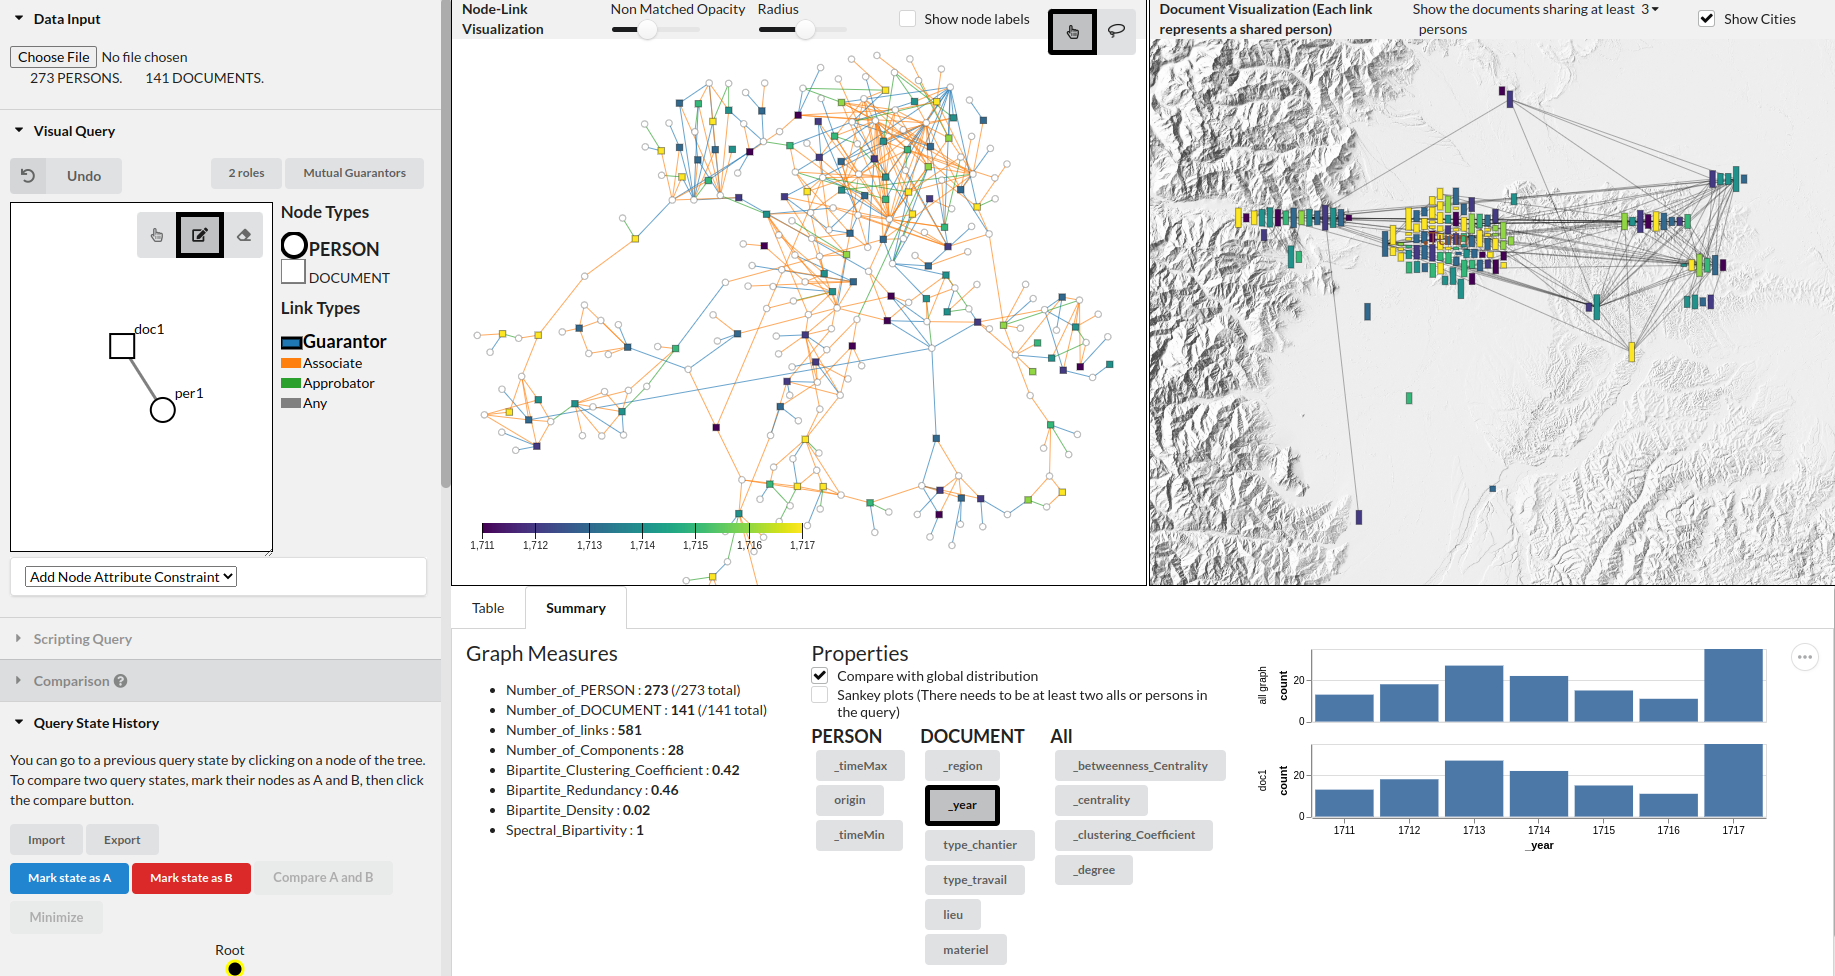
\includegraphics[trim={15.9cm 0 0 0},clip,width=\textwidth]{static/figures/ComBiNet/Piemont_timeSelected.png}
    \caption{\name interface wreal-timeith the dataset of collaboration \pascal. The user selected the \textit{\_year} attribute, showing the distribution of document years with a histogram (bottom right), and coloring the documents node on the bipartite view (left) and map view simultaneously (right).}\label{fig:combinet-time-selected}
\end{figure}

\subsection{Query Panel}

The query panel allows users to rapidly build queries visually, with topological and attribute constraints.
The visualization of the query is synchronized with the Cypher query sent to the database.
Modifying one representation update the other, allowing users to build a query visually and refine it in Cypher when appropriate.
Experts users who know the Cypher language can also start to construct their query textually and modify it visually later on.
In this subsection, I describe all the features and interactions allowing \name to build a query and illustrate them with questions 2 and 6 of our collaboration \pascal.
Our collaborator wants to \textit{find the persons who are mutually guarantors to each other in separate contracts (2)} and to know \textit{how Torino and Torino's surroundings differ according to their contracts (6)}.
\autoref{fig:visualQueriesExamples} (left) shows the final queries, but first, I explain how to create them.
?
\noindent\textbf{V6: Node-Link Dynamic Query}
% \todo{talk about the different links types, ego networks and paths, lasso}

The interactive node-link diagram allows the construction of a subgraph query graphically, that represents a topological constraint (T2.1).
The query subgraph is built and edited interactively.
At each modification, the visual query is converted into a Cypher query and run in the database which returns the results.
All the matches are displayed in the entities tables (V3) and highlighted in the main visualization views (V1, V2).
Three modes of interaction are available through the top-right menu: \textit{selection, addition}, and \textit{deletion}.
The \textit{selection} mode allows to drag the nodes in the panel, while the \textit{addition} and \textit{deletion} modes allow the following actions:
\begin{description}
    \item[\textbf{Node Creation:}] In \textit{addition} mode, clicking on an empty area creates a new node. The node will be of the selected type from the legend on the right (Person or Document).
    \item[\textbf{Node Deletion:}] In \textit{deletion} mode, clicking on a node deletes it and its links.
    \item[\textbf{Change Node type:}]  In \textit{selection} mode, clicking on a node opens a menu allowing to change its type.
    \item[\textbf{Link Creation:}] In \textit{addition} mode, clicking on a node and dragging the mouse to another node will connect the two with a link. Its type (color) will be the link type selected on the legend.
    \item[\textbf{Link Deletion:}] In \textit{deletion} mode, clicking on a link deletes it.
    \item[\textbf{Change link type:}] In \textit{selection} mode, clicking on a link opens a menu to change its type.
\end{description}

Users build concrete subgraphs with the same representation as in the bipartite network view: a visual query is a network template with additional attribute constraints.
Each role (link type) is rendered using a color (\autoref{fig:linkTypes} left).
Users can also create untyped links using the \textit{Any} value, which will match all the existing link types (\autoref{fig:linkTypes} left).
Created links can be matched by different selected link types, by checking several possible types for one link.
These links are represented by a dashed line with the colors of the possible types (\autoref{fig:linkTypes} middle right).
Several links with different types can also be created among two nodes to query a person with more than one role in the same event (\autoref{fig:linkTypes} right).
%All possibilities for link creation are shown in \autoref{fig:linkTypes}.
When a node or link is created in the query, it is given an identifier starting with \emph{per} for a person, \emph{doc} for a document, \emph{link} for a link, followed by a number.
These identifiers are used in the attribute constraint panels and the textual query and can be changed through their textual representations.


\begin{figure}[!ht]
    \centering
    % \begin{overpic}[width=0.6\linewidth]{static/figures/ComBiNet/OriginalPaperFigures/links/allLinks.pdf}
    % \end{overpic}
    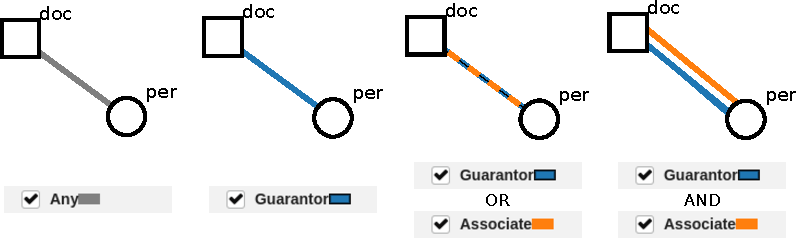
\includegraphics[width=0.9\linewidth]{static/figures/ComBiNet/OriginalPaperFigures/CGF/links.pdf}
    \caption{All link creation possibilities: Any link type (left), one selected link type, here guarantor (middle left), the union of several link types (middle right), several links with different types (right)}\label{fig:linkTypes}
\end{figure}

To find persons who are mutually guarantors in our collaboration \pascal, we first create one person and two documents using the addition mode and by clicking on the canvas.
We then link the person node to the first document with a link that is not typed (\autoref{fig:linkTypes} left), and link it to the second document with a \textit{guarantor} link (\autoref{fig:linkTypes} middle left).
We then create a second person node and link it to the two documents with opposite link types.
The resulting visual query is presented in \autoref{fig:visualQueriesExamples} (a).
To answer question 6 (comparing Torino and Torino surroundings), we start to request all the links in the graph, no matter the type, as shown in \autoref{fig:visualQueriesExamples} (b).
The database then returns all the links in the graph with their attached nodes.
Putting attribute constraints on the location of the contracts will then let us answer the question.



\begin{figure}[!ht]
    \centering
    \begin{subfigure}[b]{0.29\linewidth}
    \centering
    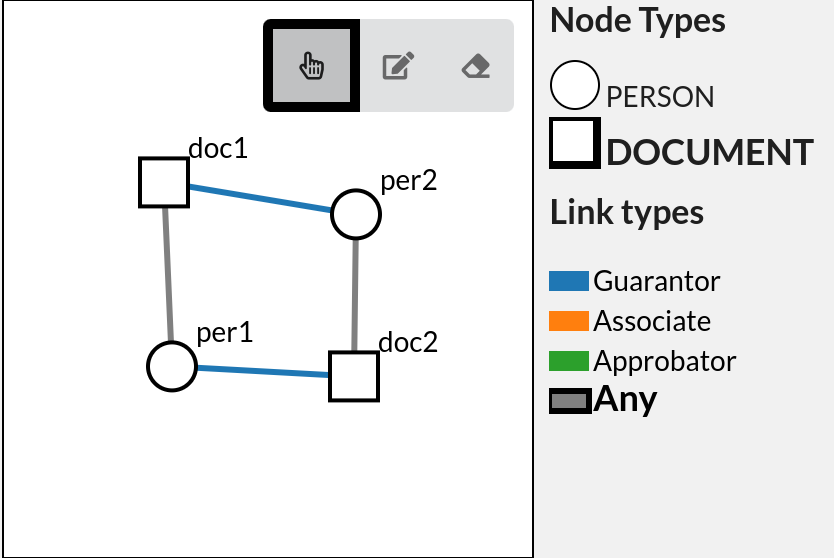
\includegraphics[width=\textwidth]{static/figures/ComBiNet/OriginalPaperFigures/CGF/MutualGuarantors.png}
    \caption{}
    \end{subfigure}
    \begin{subfigure}[b]{0.70\linewidth}
    \centering
    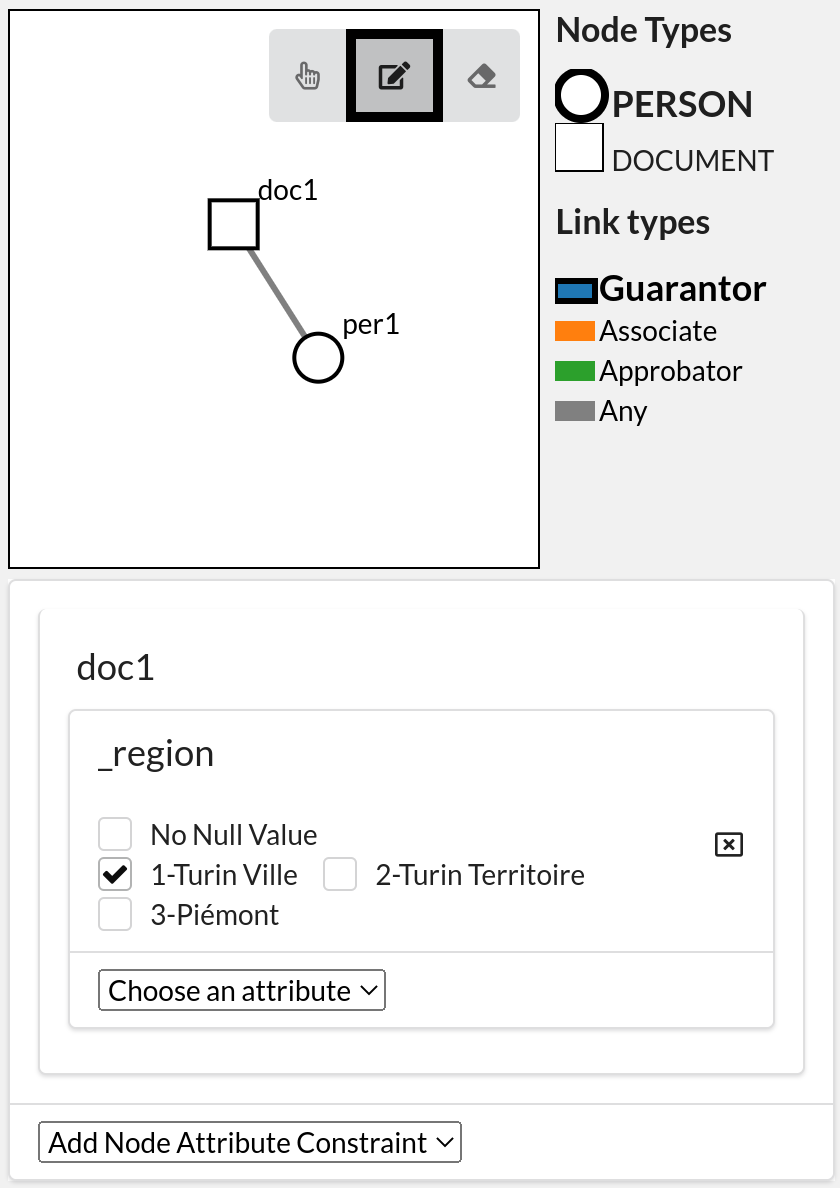
\includegraphics[width=0.46\textwidth]{static/figures/ComBiNet/OriginalPaperFigures/CGF/Turin.png}
    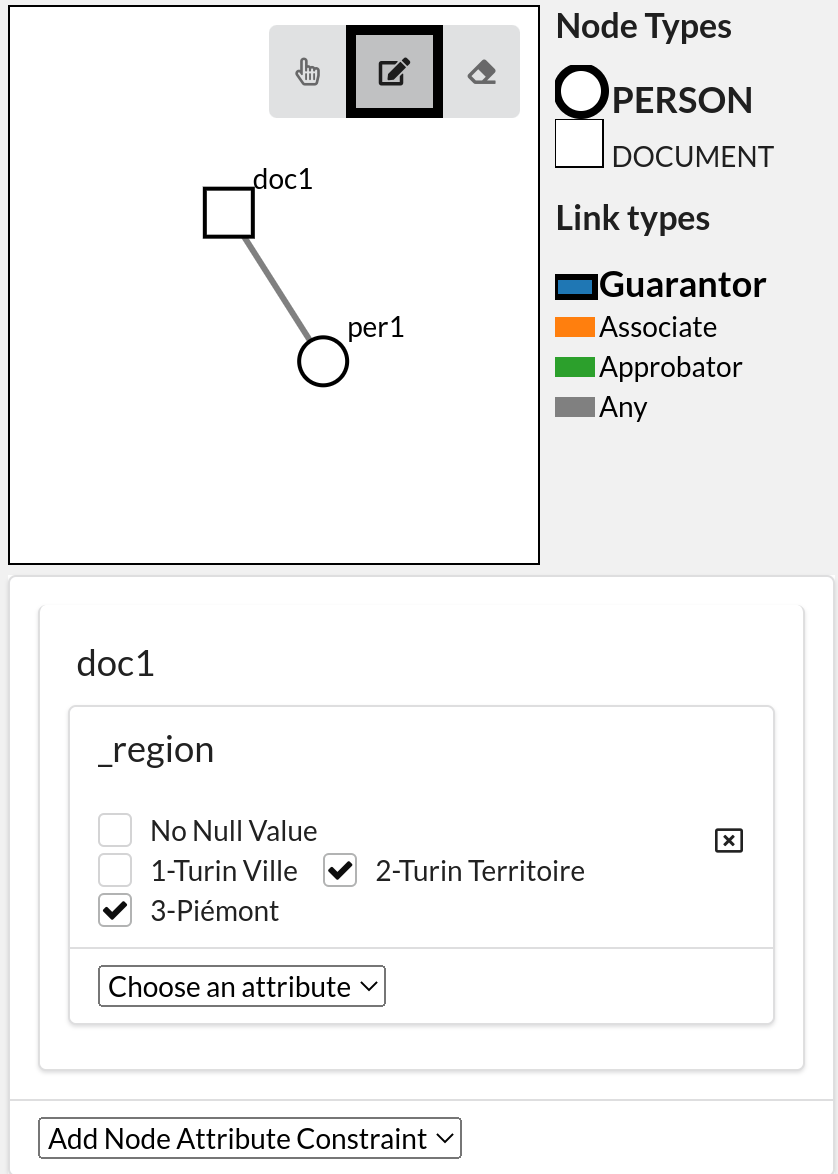
\includegraphics[width=0.46\textwidth]{static/figures/ComBiNet/OriginalPaperFigures/CGF/TurinoSuburbs.png}
    \caption{}
    \end{subfigure}

    \caption{Visual queries created to answer questions 2 and 6 of our collaboration \pascal. (a) The visual query retrieves individuals who are mutually guarantors to each other in separate construction contracts.
        (b) The two visual queries retrieve the documents---along with the signatories---of Torino (\textit{Turin} in french) (left) and of Torino surroundings (\textit{Turin Territoire} and \textit{Piemont}) (right)}\label{fig:visualQueriesExamples}
\end{figure}


%\iffalse
%\begin{figure}
%    \centering
%
%    \begin{overpic}[trim=60 60 60 60, width=0.2\linewidth]{static/figures/ComBiNet/OriginalPaperFigures/NL01}
%    \put(55, 12) {\circled{1}}
%    \end{overpic}
%    \begin{overpic}[trim=60 60 60 60, width=0.2\linewidth]{static/figures/ComBiNet/OriginalPaperFigures/NL02}
%    \put(55, 12) {\circled{2}}
%    \end{overpic}
%    \begin{overpic}[trim=60 60 60 60, width=0.2\linewidth]{static/figures/ComBiNet/OriginalPaperFigures/NL03}
%    \put(55, 12) {\circled{3}}
%    \end{overpic}
%    \begin{overpic}[trim=60 60 60 60, width=0.2\linewidth]{static/figures/ComBiNet/OriginalPaperFigures/NL04}
%    \put(55, 12) {\circled{4}}
%    \end{overpic}
%
%    \caption{Steps to create a new node and link in the node-link diagram. 1: Initial query of one document. 2: Creation of one person node by click. 3: Creation of one Approbator (marked A, green link) link by click and drag. 4: The link between the document and the person has been created after mouse release.}\label{fig:NodeLinkCreation}
%\end{figure}
%\fi



\noindent\textbf{V7: Attribute Constraint Widgets}\label{sec:attributes}
Users can also add attribute constraints (T2.2) on the created nodes with the help of interactive widgets.
An input button is created for each node and link identifier from the node-link query panel.
It allows the creation of a dynamic query widget for any of its attributes.
% When selected, it initialize a constraint visualized by a widget users can interactively modify.  The possible choices of attributes depend on the node type (person or document).
The widget design varies according to the three possible attribute types: numeric, categorical, and nominal, as in the original dynamic queries formalization by Shneiderman~\cite{DynamicQueries}:
\begin{enumerate}
    \item \textbf{Numeric constraints} are modeled as range sliders, allowing the selection of lower and upper bounds to the filter.
    \item \textbf{Categorical constraints} are modeled as a set of checkboxes. Each possible value has a corresponding checkbox.
    \item \textbf{Nominal constraints} are modeled as text input, where the user can write any desired value. All the possible values are shown at the same time and filtered as the user writes.
\end{enumerate}

For the categorical and nominal widgets, selecting several values corresponds to the union of the filters.
The three widget types are shown in \autoref{fig:combinet-widgets}.

\begin{figure}[!ht]
    \centering
%    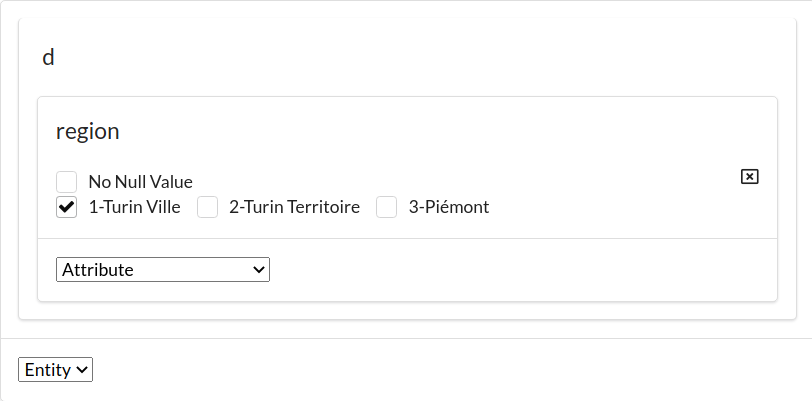
\includegraphics[trim=30 145 300 110,clip,width=0.8\linewidth]{static/figures/ComBiNet/OriginalPaperFigures/constraintRegion.png}%
    % 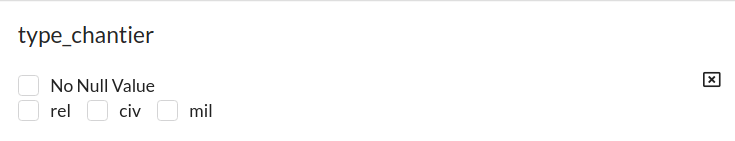
\includegraphics[width=0.8\linewidth]{static/figures/ComBiNet/OriginalPaperFigures/categoricalWidget}
    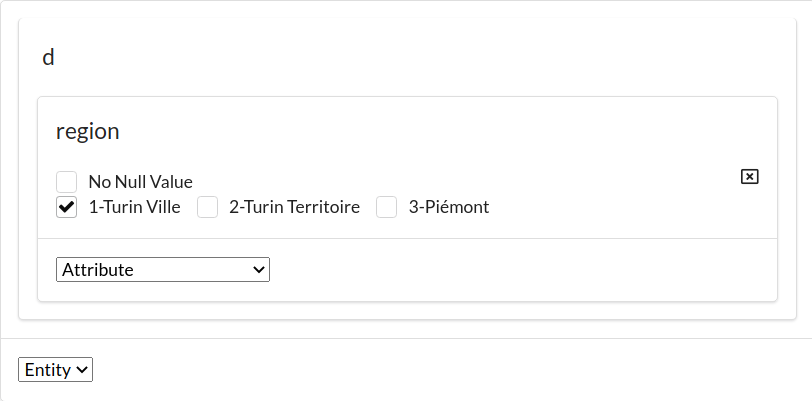
\includegraphics[width=0.7\linewidth]{static/figures/ComBiNet/OriginalPaperFigures/constraintRegion.png}\\
    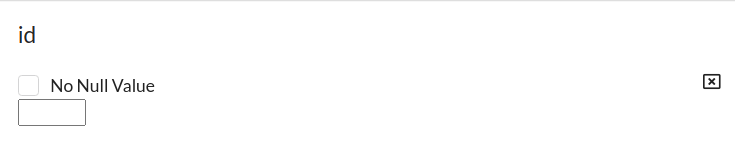
\includegraphics[width=0.6\linewidth]{static/figures/ComBiNet/OriginalPaperFigures/nominalWidget}\\
    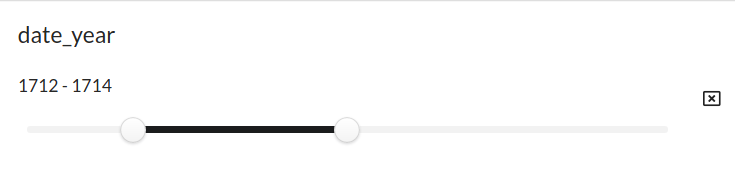
\includegraphics[width=0.6\linewidth]{static/figures/ComBiNet/OriginalPaperFigures/numericWidget}

    \caption{Widget designs for the different attribute types: checkboxes for categorical attributes (top), text input for nominal attributes (middle), and a double slider for numerical attributes (bottom). The categorical attribute example shows the  inputs letting users create new constraints for other attributes and other nodes.}\label{fig:combinet-widgets}
\end{figure}
%\fi

To answer our collaborator's second question (\textit{how do Torino and Torino's surroundings differ according to their contracts?}), we first filter the documents which are located in Torino (\textit{Turin}).
For this, we select the whole dataset by linking a person and document node with an untyped link.
Then, we select the id \textit{doc1} of the document of our visual node-link query, and the \textit{region} attribute.
It initializes a categorical widget including all the values found in the dataset for this attribute with associated checkboxes.
We check the region of interest ``\textit{1-Turin Ville}'' to select all the documents from this region.
 The first widget of \autoref{fig:combinet-widgets} illustrates the created constraint.
To select the documents of Torino's surroundings, we can simply uncheck the ``\textit{1-Turin Ville}'' value for the \textit{region} attribute and check the two other values ``\textit{2-Turin Territoire}'' and ``\textit{3-Piemont}'' which are areas corresponding to the surroundings of Torino.
Both queries are represented in \autoref{fig:visualQueriesExamples} (b).


\noindent\textbf{V8: Cypher Editor}
Users can build or modify a query using the Cypher query language, with the Cypher text editor.
This allows users to start creating a query visually and refining it by text for complex constraints which can not be represented by a visual form easily.
The parts of the Cypher query which are not visually expressible appear in Cypher widgets next to the other widgets.
The editor supports autocompletion e.g., to help to discover and spell the attribute names.
The visual and textual representations are synchronized, meaning that modifying one update the other and return the results in the visualizations, tables, and attribute distributions.


\noindent\textbf{Query Results}

Each modification of the query, whether from the node-link dynamic query, the widgets, or the Cypher text box, update the two visualization panels (V1, V2), the entities tables (V3), the network measures view (V5), and the attribute plots (V6).
The nodes and links that do not match (are not retrieved by the query) are grayed out in V1 and V2 and are removed from the persons and documents tables (V3).
A third table shows every occurrence found of the created pattern that we call the occurrence table.
The occurrence table for question 1 of collaboration \pascal is shown in \autoref{fig:combinet-example-results} (a).
It tells us that the occurrence has been found 72 times, meaning that the pattern exists 36 times in the network by taking into account the symmetry of the subgraph query.
Users can switch between the three tables in the table view using the tabs.
The network measures are computed on the new subgraph formed by the union of all patterns found and updated on the network measures view (V5).
\autoref{fig:combinet-example-results} (b) (left) shows to the user the different graph measures of the subgraph induced by the patterns found.
Since some measures can be long to compute, the values are computed iteratively in the backend and shown progressively~\cite{feketeProgressiveDataAnalysis2019} to avoid blocking the interface.
The distribution plots in the attributes view (V6) are updated, showing the values of the entities of the latest constructed query, next to the global distributions.

%By selecting the \textit{origin} attribute as seen in \autoref{fig:combinet-example-results} (b) (right)

% Each modification of the query, whether from the node-link dynamic query, the widgets, or the Cypher text boxes, update the two visualization panels. The nodes and links that do not match (are not retrieved by the query) are grayed out. It allows to rapidly visualize the subset of entities resulting from the applied query while maintaining the context.
% The results are shown in detail in the results section panel, constituted of the results tables and summary tabs, both shown in \autoref{fig:ResultsSection}. The table shows each occurrence of the query pattern found in the graph, with details on demands. Clicking on a row shows every attribute of the matched entities. Users can select a set of rows to highlight and visualize the occurrences directly in the two graph views.

% The summary tab presents graph measures computed from the subgraph resulting from the union of all occurrences of the queried pattern, such as the number of persons, documents, bipartite density, and the bipartite clustering coefficient. For the specified query, 42 documents are localized in Torino, 99 persons are mentioned in these contracts 153 times (given by the number of links).

\begin{figure}[!ht]
    \centering
    \begin{subfigure}[b]{\linewidth}
        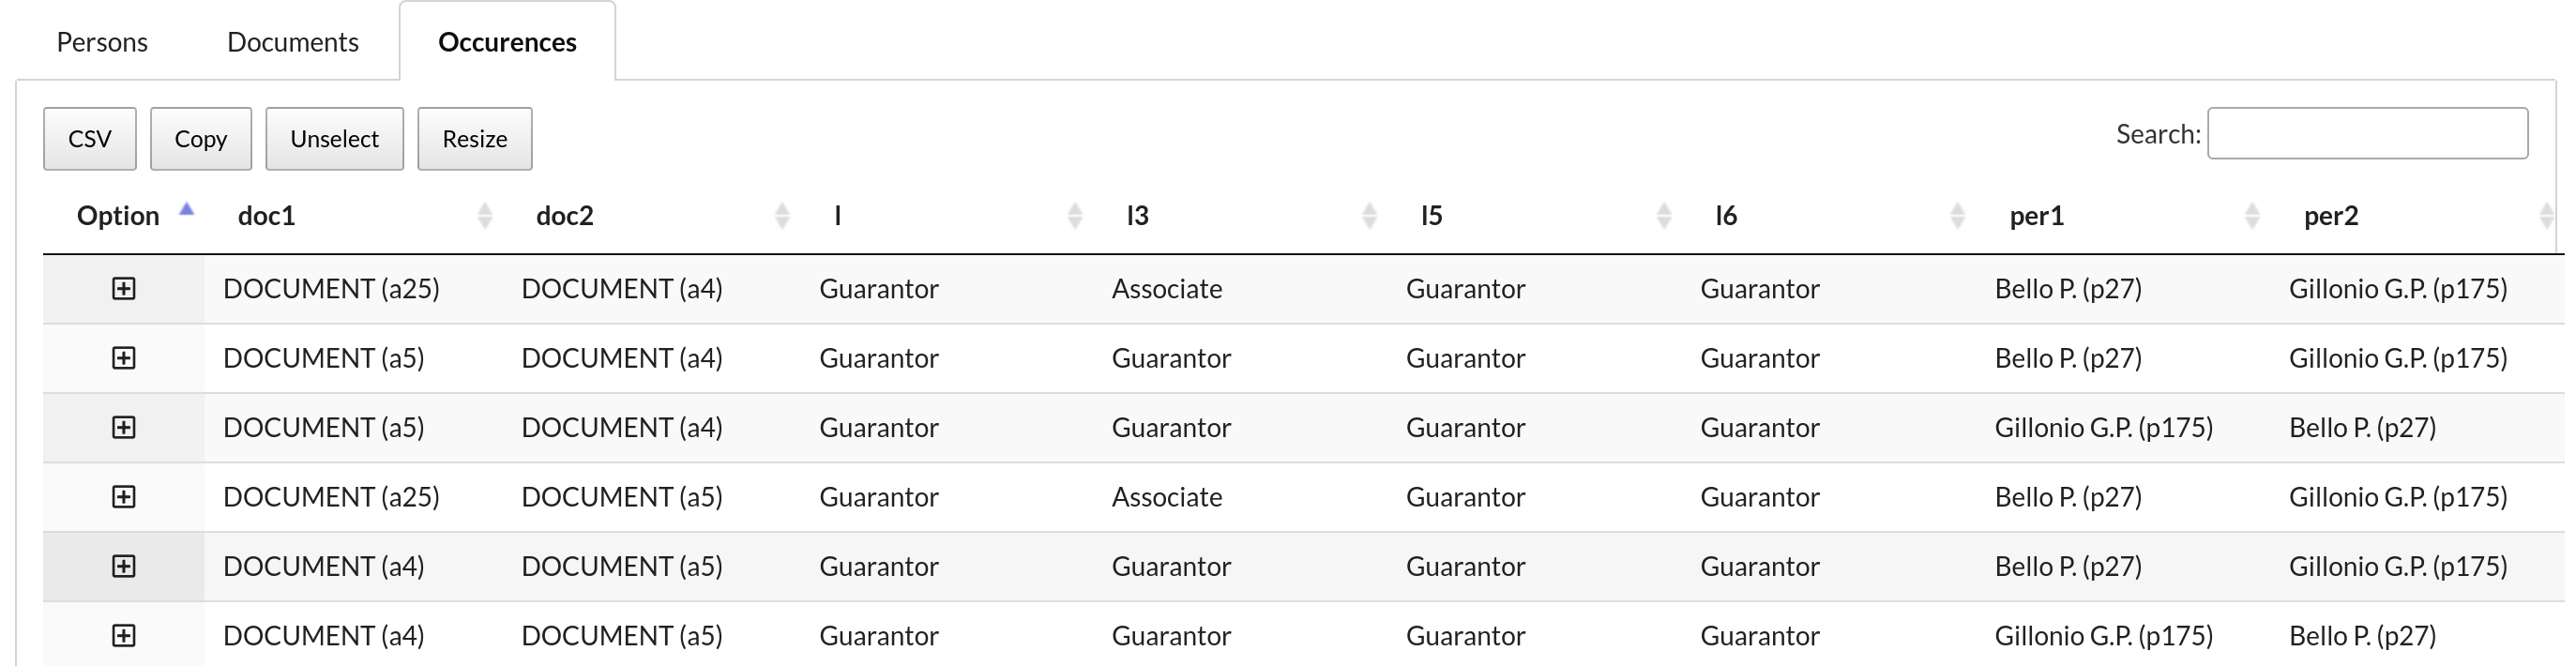
\includegraphics[width=\textwidth]{static/figures/ComBiNet/Piemont-mutual-guarantor-table}
        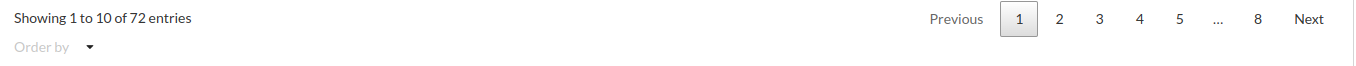
\includegraphics[width=\textwidth]{static/figures/ComBiNet/mutualGuarantor-table-bottom}
    \caption{}
    \end{subfigure}

    \begin{subfigure}[b]{\linewidth}
            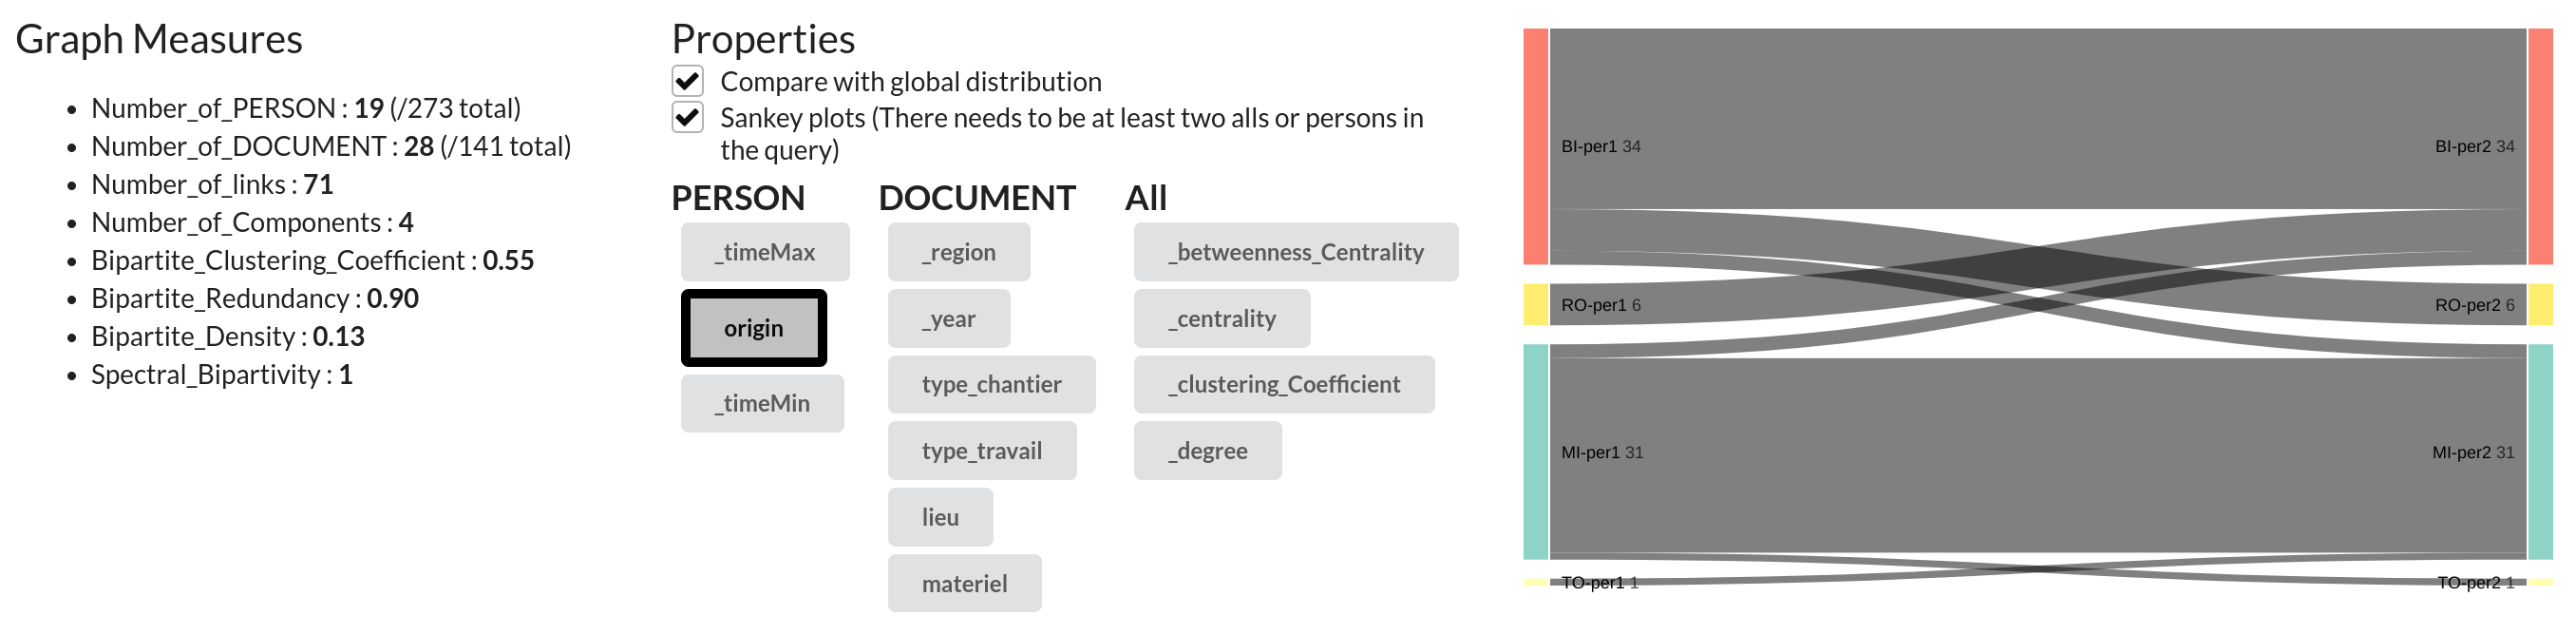
\includegraphics[width=\textwidth]{static/figures/ComBiNet/piemont-mutual-guarantors-results}
    \caption{}
    \end{subfigure}

    \caption{Results of question 2 of collaboration \pascal: (a) shows a subset of the table view with every occurrence of the pattern found. (b) shows the summary panel, with the graph measures and the attributes view with the \textit{origin} attribute selected and the Sankey option checked. It allows us to see the attribute distribution of the persons included in the pattern and see if there is a relationship between persons who are mutually guarantors and their origin.
%    bioglio BI
%    Comune di Ro
%    MI Milano
    }\label{fig:combinet-example-results}
\end{figure}


\noindent\textbf{Attributes Visualization} When users select an attribute in the attributes view (V5), its distribution is visualized for the queried entities and the whole network with a histogram.
However, these plots show the aggregated values and we lose the potential value transitions between the query nodes.
For example, \autoref{fig:sankeys} shows a query to list the persons with the role of ``approbator'' (green) in a contract after being a ``guarantor'' (blue) in another contract (using a time constraint).
We may want to see if the locations or types of the two contracts are the same or if they change, case by case.
Unfortunately, we lose this information with the aggregated plots.
By checking the ``Sankey'' option on top of the distribution visualization, the plots are transformed into Sankey diagrams, giving information on how the attribute values relate between the nodes (person or event) of the same query.
% The given query example along the distribution of the \textit{type chantier} in both a stacked bar chart and Sankey diagram is shown in .
A Sankey diagram showing the attribute distributions is particularly useful for queries where nodes have a relationship in regard to time, such as birth certificates, marriage, or death certificates where we know the order in which these events occurred.
It is also useful for queries with user-defined time order constraints as in \autoref{fig:sankeys}.

The attribute plots are exportable in SVG, while the tables are exportable in CSV, pdf, or directly in the clipboard.
%The tables are exportable in csv, pdf, or directly in the clipboard while the attribute plots are exportable in SVG.
This was a demand of our collaborators, who can share the results of their queries easily or use them in another software or tool, according to the \emph{traceability} principle.

\begin{figure}[!ht]
    \centering

    \begin{subfigure}[b]{0.24\linewidth}
    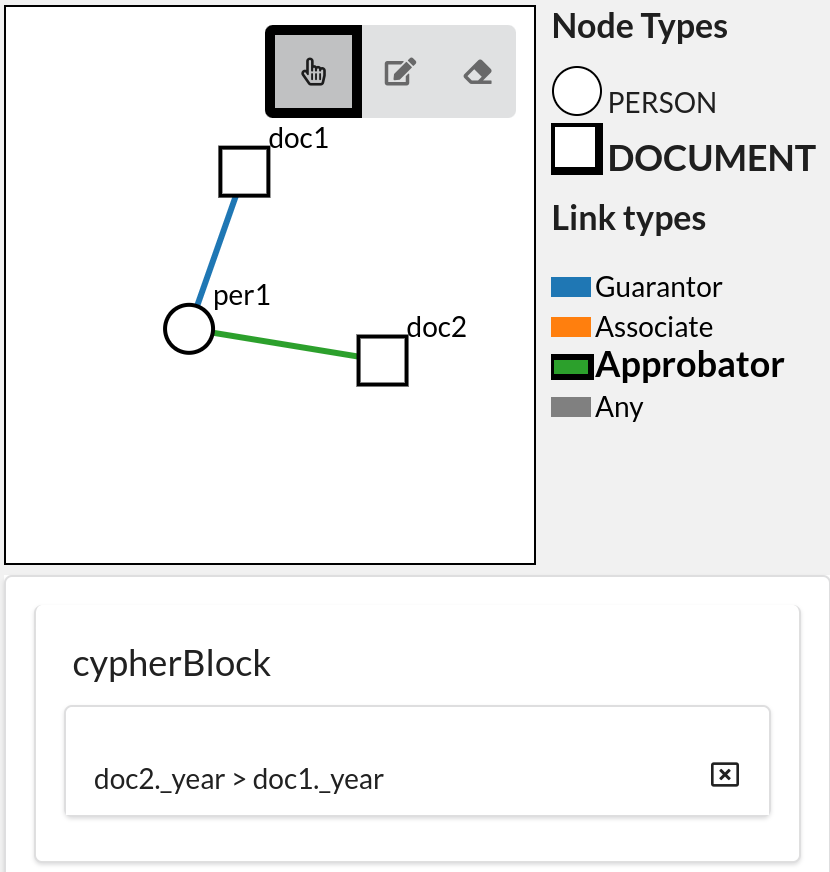
\includegraphics[width=\textwidth]{static/figures/ComBiNet/OriginalPaperFigures/CGF/sankeyPLot/apprGuar.png}
    \caption{}
    \end{subfigure}
    \begin{subfigure}[b]{0.3\linewidth}
    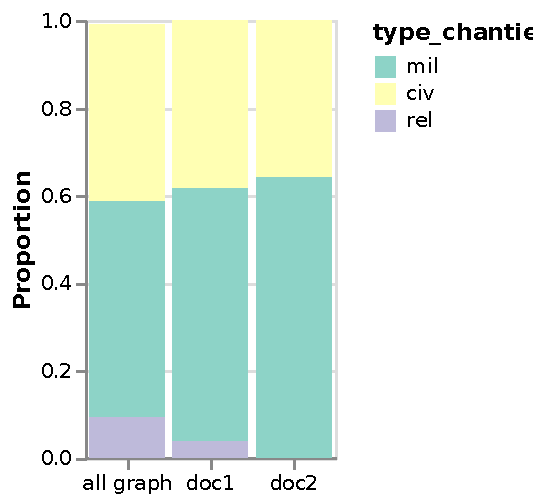
\includegraphics[width=\textwidth]{static/figures/ComBiNet/OriginalPaperFigures/CGF/sankeyPLot/barchart.pdf}
    \caption{}
    \end{subfigure}
    \begin{subfigure}[b]{0.44\linewidth}
    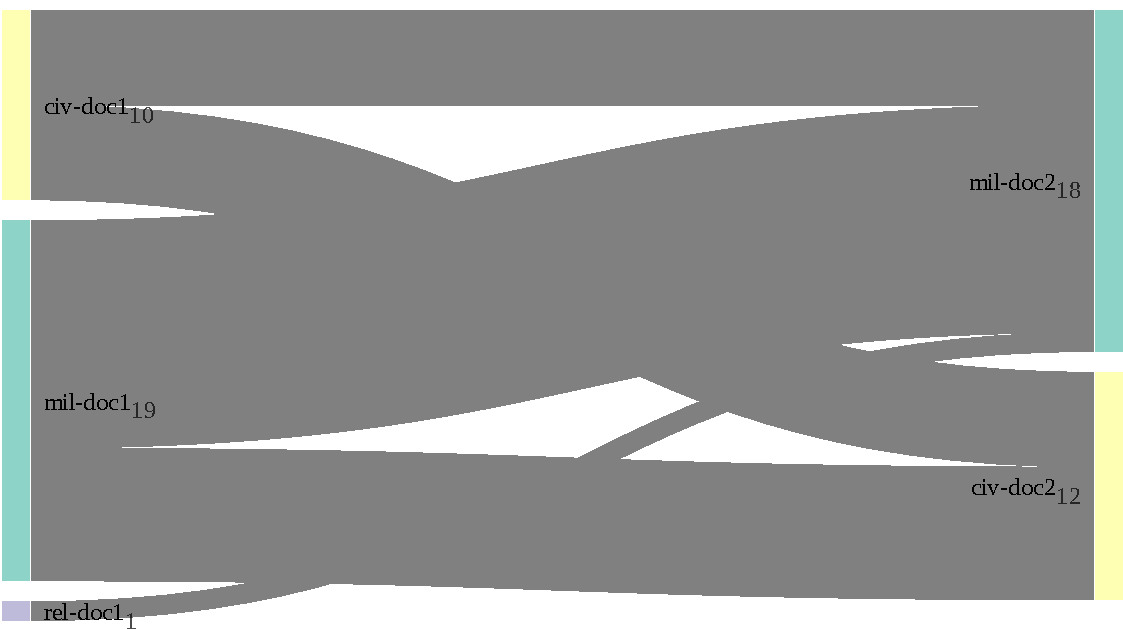
\includegraphics[width=\textwidth]{static/figures/ComBiNet/OriginalPaperFigures/CGF/sankeyPLot/sankey_bigger.pdf}
    \caption{}
    \end{subfigure}
    \caption{Two ways of showing the distribution of ``type chantier'' (type of works), a categorical attribute with three possible values ``\textsl{rel}igious'', ``\textsl{mil}itary'', and ``\textsl{civ}ilian''.
    (a) A query matching the contracts made by the same person (\textit{per1}) as an ``approbator'' (green link to \textit{doc2}) after being a ``guarantor'' (blue link to \textit{doc1}) using the constraint (\texttt{doc2.\_year > doc1.\_year}). (b) Stacked bar chart for the matches, the earlier contract (\textit{doc1}), the older contract (\textit{doc2}), and (c) Sankey diagram with the early values on the left and the last on the right.
    The Sankey diagram reveals the value changes between the two documents: the guarantor who worked initially on religious work switched to military work.} \label{fig:sankeys}
\end{figure}

The graph measures and attribute views for the results of question 2 of collaboration \pascal are shown in \autoref{fig:combinet-example-results}.
The Sankey view of the \textit{origin} attribute shows that mutual guarantors come from 4 regions only and that usually, people have mutual guarantor relationships only with persons of the same origin.
This is especially true for persons from \textit{Milano}, and with some reciprocal links between persons from \textit{Bioglio} and the \textit{Comune di Ro}.




\noindent\textbf{V9: Provenance Tree}
Each change in the query panel is saved with the computed results so that the history of the query construction can be shown in the form of a provenance tree (T2.4), managed with the Trrack library~\cite{cutlerTrrackLibraryProvenanceTracking2020}.
Each node of the tree represents a query change, with a descriptive label such as ``New Link''.
It enables to rapidly visualize the succession of filters applied with their refinements.
At any moment, users can rename a tree node or click on it to go back to the previous state; allowing them to explore different query possibilities easily and iteratively.
Hovering over a node shows a tooltip with the query panel associated with the selected query state.
It let users rapidly see what query is associated with each node of the tree
If a new change is made on the query from a previous state, a new branch is created on the tree, permitting to revisit and refine explorations.  \autoref{fig:combinet-trees} shows the provenance tree made to answer question 2, split into 2 branches, with the tooltip showing one of the node query states.
\begin{figure}[!ht]
     \centering
state%     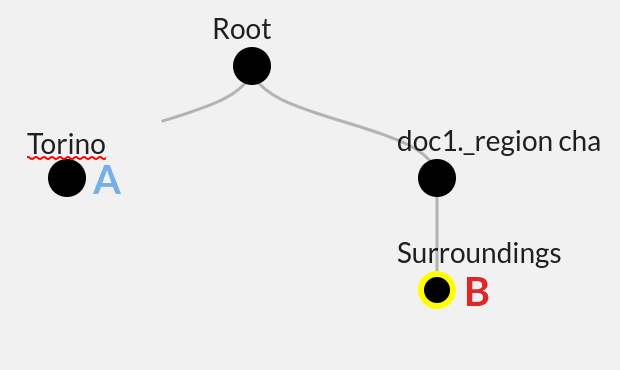
\includegraphics[width=0.3\linewidth]{static/figures/ComBiNet/torino_tree}
     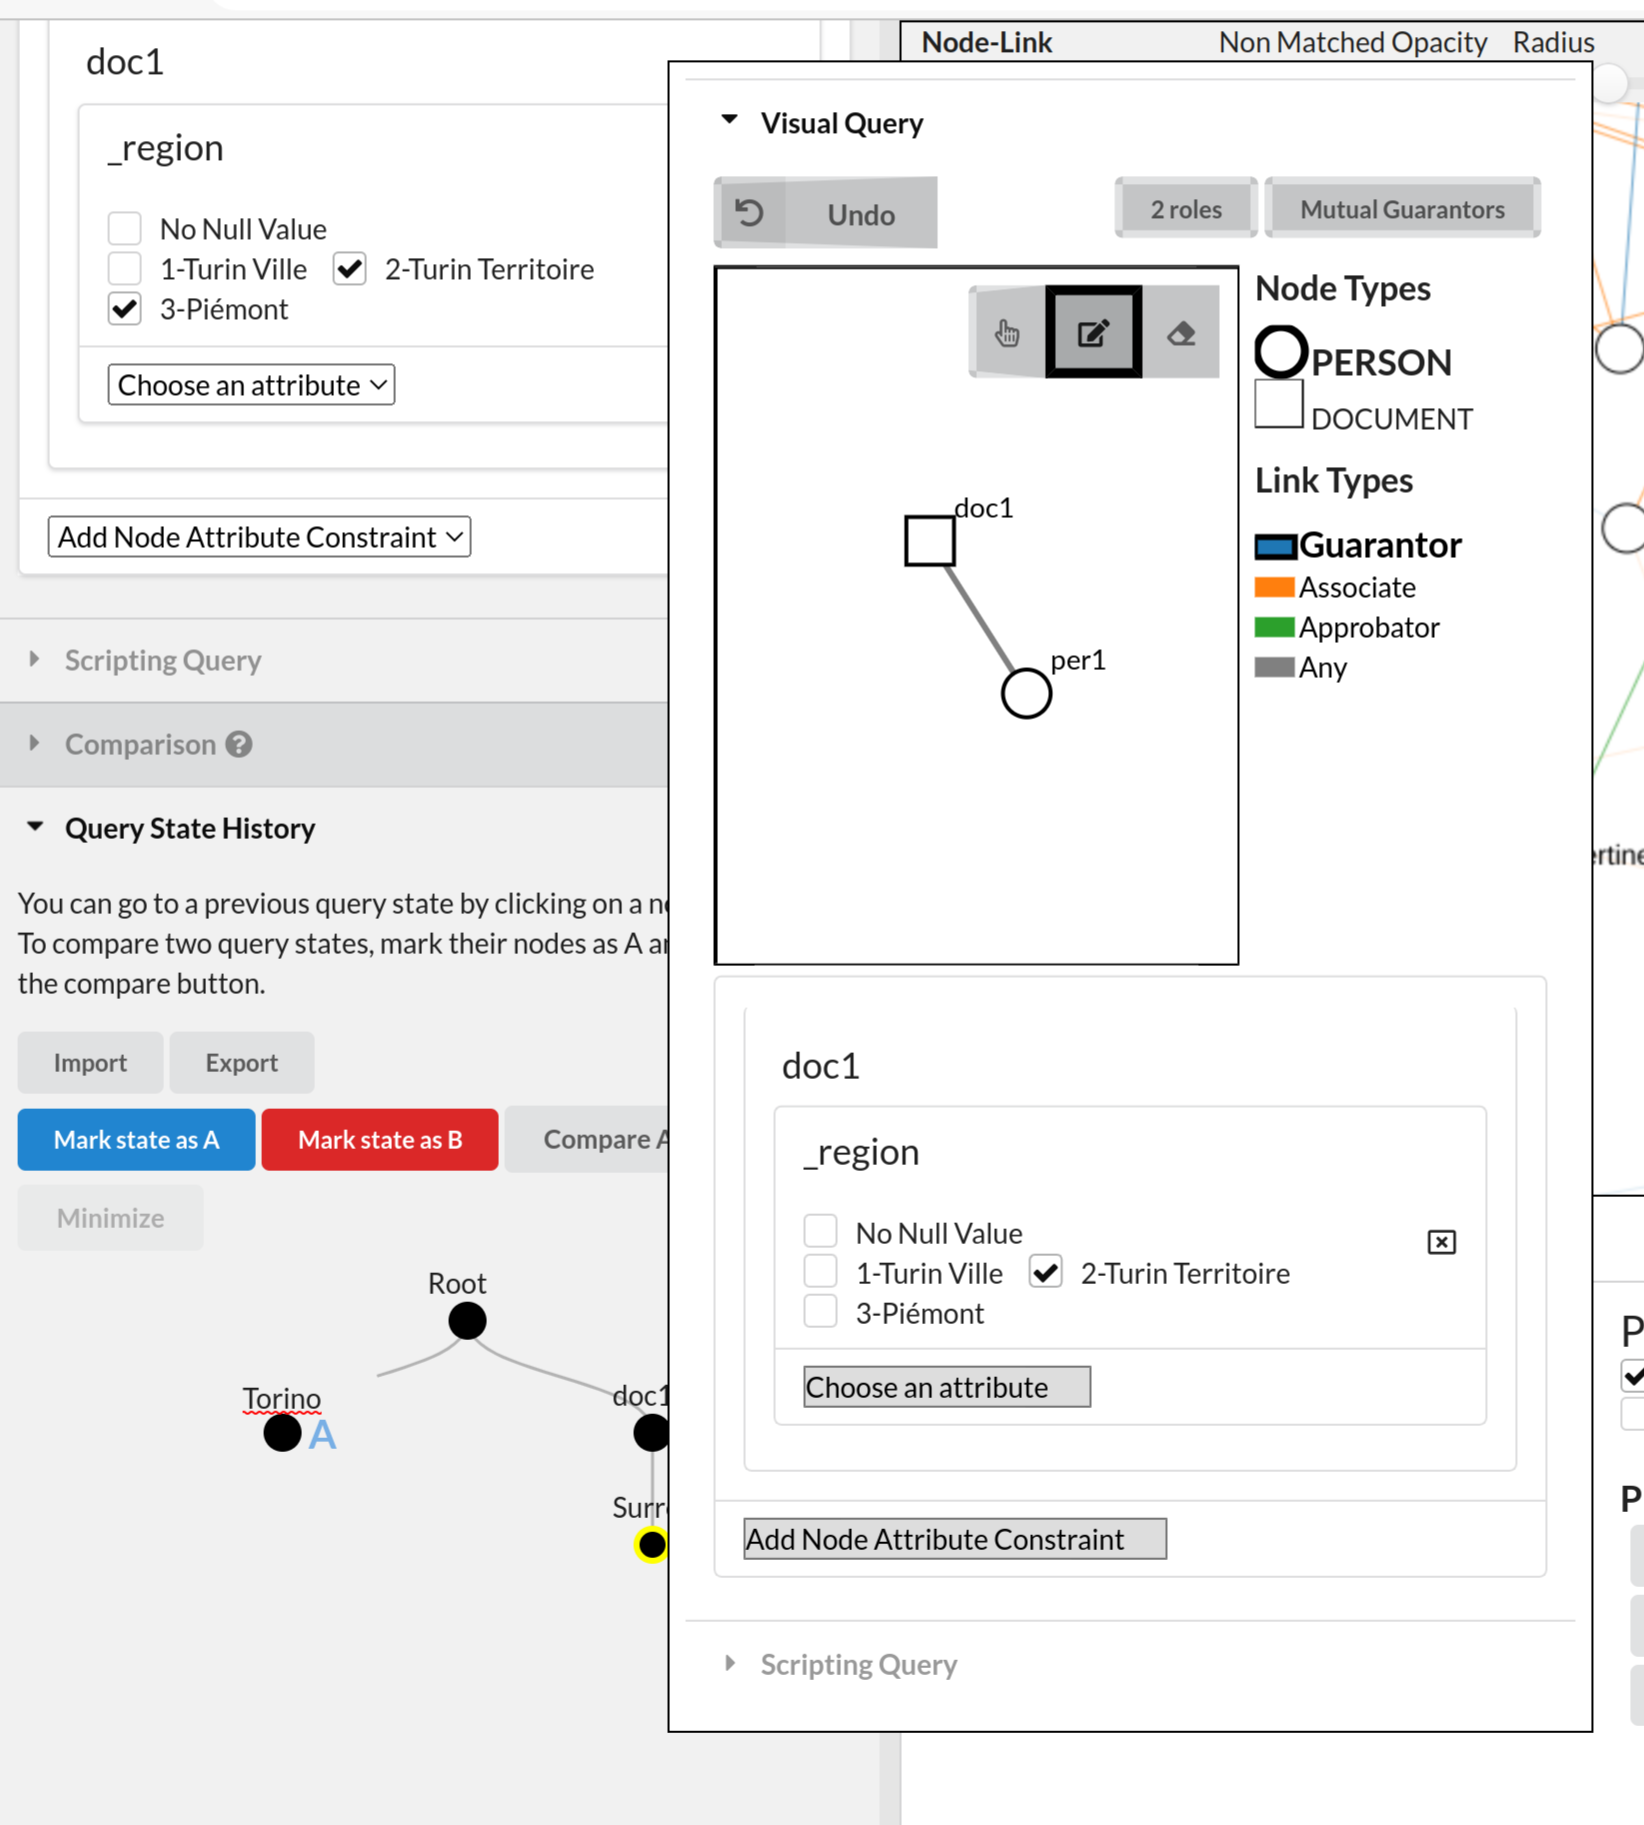
\includegraphics[width=0.5\linewidth]{static/figures/ComBiNet/tree_tooltip_torinoquery_crop}
%     \caption{(a) Provenance tree to answer question 2 of collaboration \pascal: left branch lead to Torino documents (the node is labeled as A) while right branch lead to surrounding documents (the node is labeled as B). }\label{fig:combinet-trees}
     \caption{Provenance tree to answer question 2 of collaboration \pascal: left branch leads to Torino documents (the node is labeled as A) while right branch leads to surrounding documents (the node is labeled as B). The user hovers over one node, revealing a tooltip that shows the visualization of the node's query..}\label{fig:combinet-trees}
 \end{figure}
The whole provenance tree is exportable and importable in JSON format, allowing to 1) start a session from a previous exploration and not from scratch, 2) share exploration sessions and results with others, and 3) provide a trace of the exploration leading to a potentially interesting result, hence providing \emph{traceability} in the results.


\subsection{Comparison}

In addition to comparing the results of a query to the whole graph, \name allows comparing the results of two queries.
Users can select two query states in the provenance tree and mark them either as ``A'' or ``B''.
Clicking on the button ``Compare State A and B'' compares them.
The interface changes to \emph{comparison mode}.
Several buttons appear on top of the provenance tree: $A$, $B$, $A-B$, $B-A$, $A \cap B$, and $A \cup B$ for exploring the combinations of the two results of A and B in the two visualizations panels.

To answer several of the questions raised by our collaborators, we need to compare two subsets of the network.

In question 6 of collaboration \pascal, we want to compare the constructions in Torino with the ones in Torino surrounding.
Since we previously constructed the query returning all the contracts from Torino (\textit{Turin}) with the mentioned people, we can
return to this point in the provenance tree, and change the constraint of the \textit{region} attribute from \textit{Turin} to \textit{Turin Territoire} and \textit{Piemont} using the checkboxes to get the documents of Torino surroundings in a second query.
Both queries are shown in \autoref{fig:visualQueriesExamples} (b).
The user can then rename the provenance tree nodes with explicit names such as ``Torino'' and ``Surroundings'', and mark them as A and B using the appropriate buttons.
Clicking on the ``Compare State A and B'' will make the interface compare the two query results.


% \begin{figure}
%     \centering
%     % \includegraphics[width=0.2\linewidth]{static/figures/ComBiNet/OriginalPaperFigures/query01.png}
%     % \includegraphics[width=0.2\linewidth]{static/figures/ComBiNet/OriginalPaperFigures/query02.png}
%     % \includegraphics[width=0.2\linewidth]{static/figures/ComBiNet/OriginalPaperFigures/query03.png}
%     % \includegraphics[width=0.2\linewidth]{static/figures/ComBiNet/OriginalPaperFigures/query04.png}
%     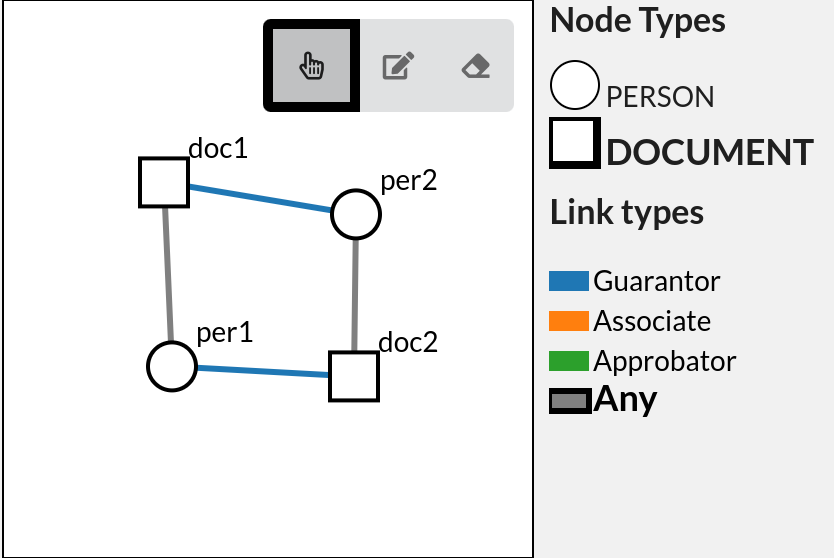
\includegraphics[scale=0.1]{static/figures/ComBiNet/OriginalPaperFigures/CGF/MutualGuarantors.png}
%     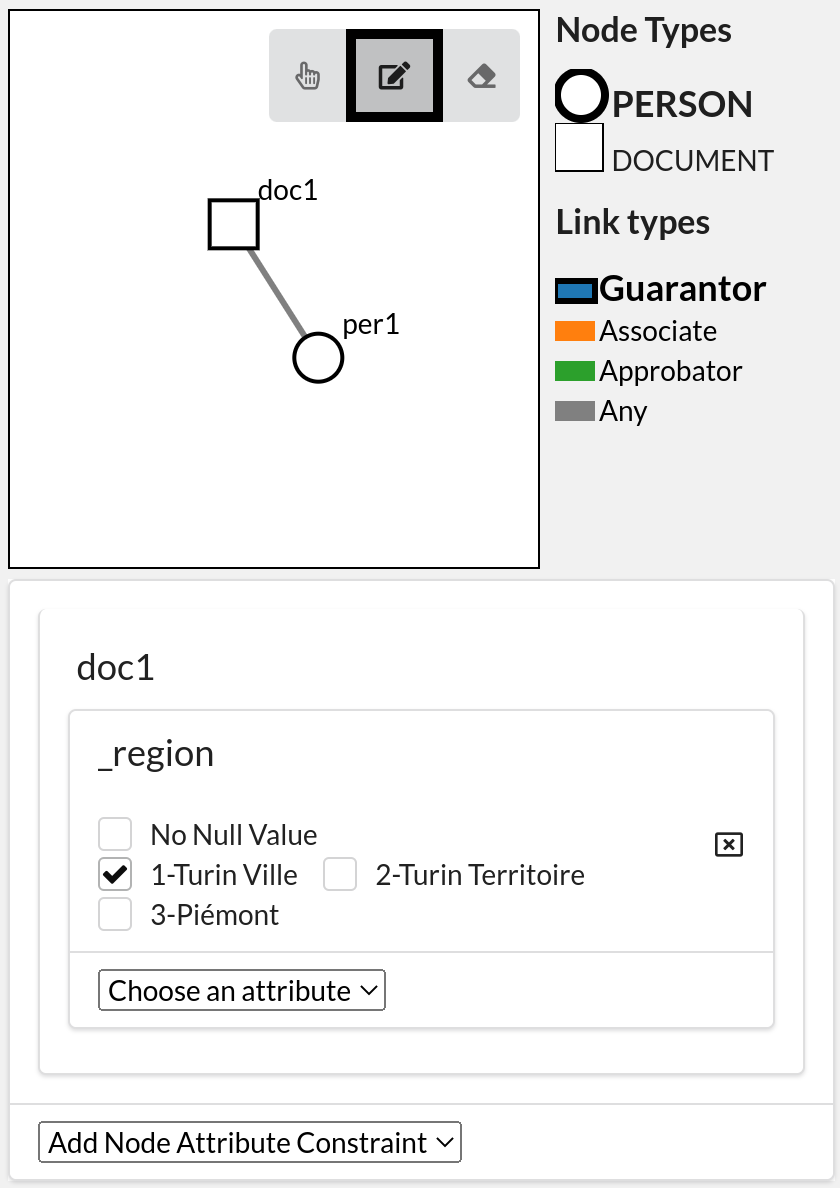
\includegraphics[scale=0.1]{static/figures/ComBiNet/OriginalPaperFigures/CGF/Turin.png}
%     \hspace{-8pt}
%     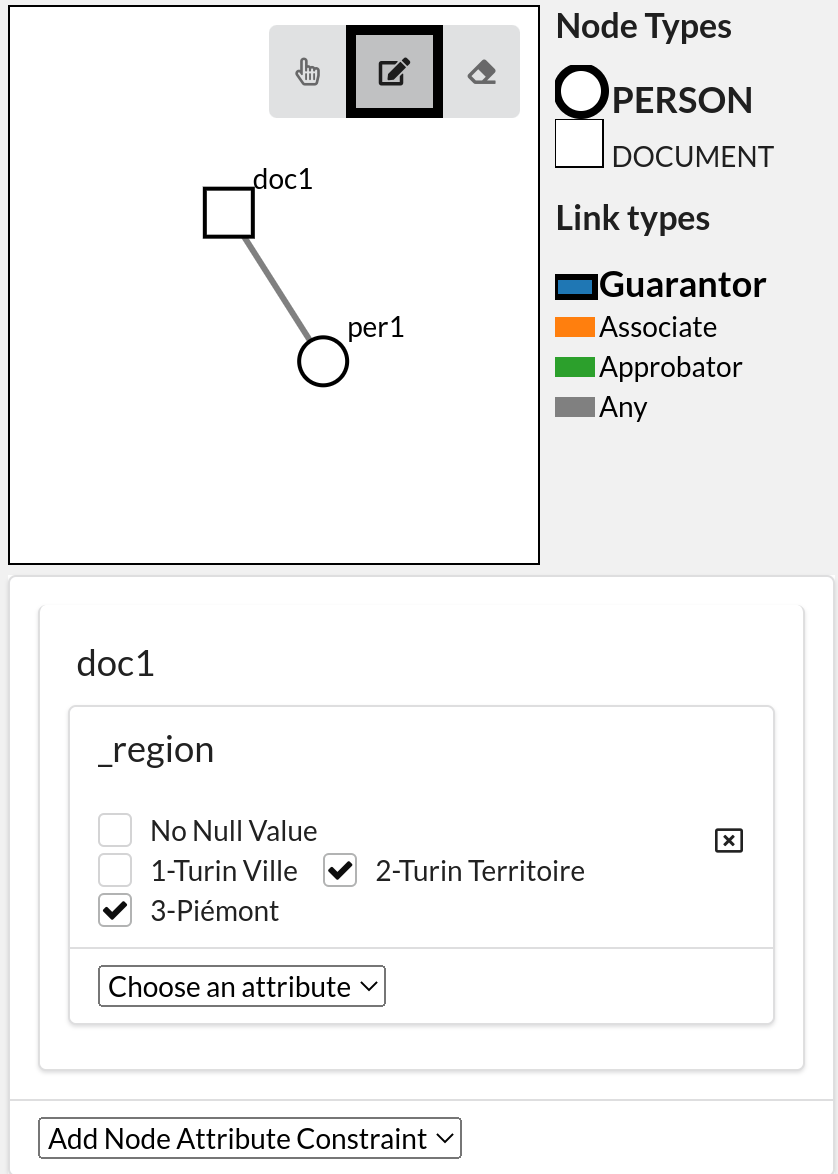
\includegraphics[scale=0.1]{static/figures/ComBiNet/OriginalPaperFigures/CGF/TurinoSuburbs.png}
%     \caption{Queries to answer our collaborator's four questions.
%     % Visual queries made to find back the four patterns our collaborator is interested in.
%     }\label{fig:queries}
%     \vspace{-8pt}
% \end{figure}

\noindent\textbf{Topological Comparison}
In comparison mode,
% the two graph visualization panels do not change but
users can rapidly switch between the visual filters of (A) and (B) by hovering over their respective buttons on the comparison menu and thus compare the structure of the two resulting subgraphs (T3.1).
Similarly, different boolean comparison operations are available by hovering their respective buttons (\autoref{fig:combinet-overall}-C), such as the intersection, union, and differences between the two filters. % It allows to rapidly change filters to find interesting persons or group of persons in a exploratory process.
Moreover, the summary tab allows comparing the different graph measures of the two subgraphs by showing them side by side (T3.3).
\autoref{fig:combinet-comparisonTable} shows the comparison table for the queries returning the subgraph of Torino (A) and Torino surroundings (B).
% as shown in \autoref{fig:comparisonTable}.
Comparing these measures, such as the number of matched documents or the densities, is crucial for \sna.
For example, the table indicates that the density is two times higher for Torino, suggesting that fewer persons participate in the same construction compared to Torino surroundings.

\begin{figure}[!ht]
    \centering
%    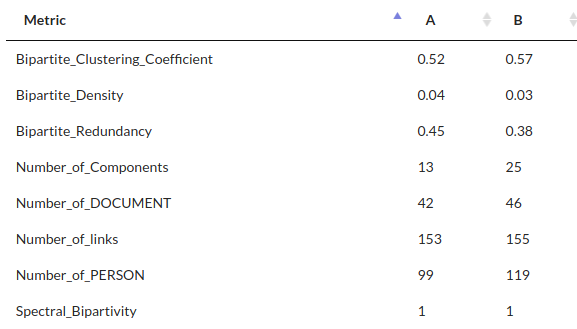
\includegraphics[width=0.8\linewidth]{static/figures/ComBiNet/OriginalPaperFigures/comparisonPlots/graphMeasuresComparison.png}
    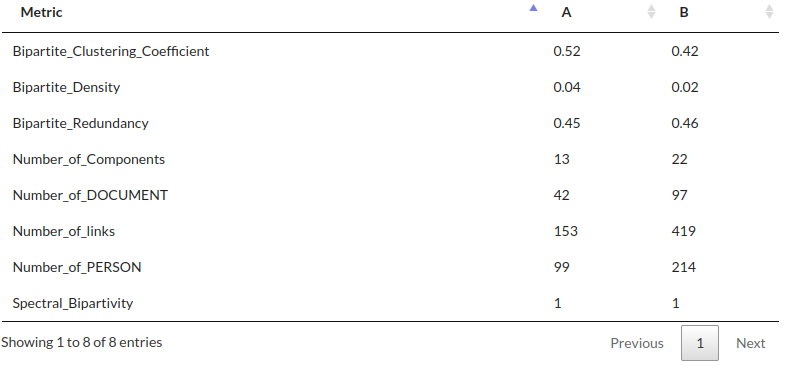
\includegraphics[width=0.8\linewidth]{static/figures/ComBiNet/graph_measures_Torino_territoireandpiemont}
  \caption{Comparison table of the network measures for Torino subgraph (A) and Torino surroundings subgraph (B).}\label{fig:combinet-comparisonTable}
\end{figure}

%\todo{comparaison de torino et territoire sur le graphe} ?

\noindent\textbf{Attribute-Based Comparison}
The comparison of one or several attribute distributions between (A) and (B) is also useful for answering the historical questions of our users.
In the attribute view (V5) of the results panel, hovering or clicking on an attribute name will show the distribution of this attribute in four contexts: the nodes of the whole graph, the queries (A), (B), and the currently selected Boolean operator (e.g., intersection or union) if one is selected.
This allows users to compare attribute distributions between several subsets of interest (T3.2).
For example, we can compare the attributes between the contracts of Torino and the ones of its surroundings.
We can also compare the persons who worked in Torino, in Torino's close territory, and in both areas, by selecting the intersection operator.
% or the persons who collaborated in those regions, if we select the intersection operator.
\autoref{fig:attributeComparison} illustrates the comparison plots for different attributes.
The first plot indicates that the types of construction sites differ between the two regions: the city of Torino clearly has a lot of military sites compared to the surroundings of Torino, which has almost none.
This is the opposite for the number of religious sites, which are almost all localized in the surroundings of Torino.
If we now look at the year distribution of the contracts, we can see a difference in the distributions.
The years of Torinos's construction contracts were steady between 1711 and 1717 with a little spike in 1713, while the constructions were more scarce in the surroundings before 1716.
We can see a big spike in construction in 1717.
This is interesting to our users, as it shows the dynamic of the construction in the area: the center of the city started to be constructed before other constructions arose in the surroundings.
%The majority of Torino's contracts occurred around 1713 and around 1717 for Torino's surroundings.

We can also compare the profiles of persons who collaborated at Torino and Torino surroundings by selecting the intersection of those two queries.
One of the questions the historian had (question 2 of \autoref{tab:tasks}) was to know if those persons were a group with specific attributes and characteristics, or were inseparable from other persons working in the two areas.
If we look at the betweenness centrality, on average, the values are higher for this group of people, meaning that the persons who work on the construction site at Torino and Torino's territory are clearly two distinct groups, and the persons collaborating in the two areas act as bridges between these groups.
This visual demonstration was convincing and revealing for our users.

\begin{figure}[!ht]
    \centering

    % 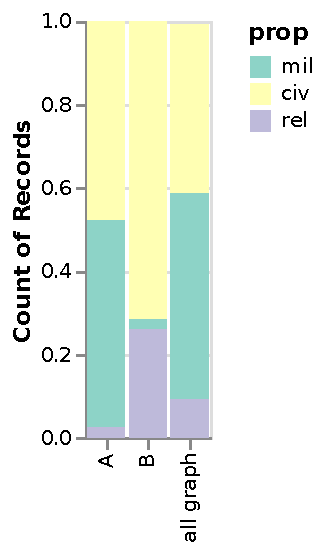
\includegraphics[width=0.2\linewidth]{static/figures/ComBiNet/OriginalPaperFigures/comparisonPlots/type_chantier}
    % % 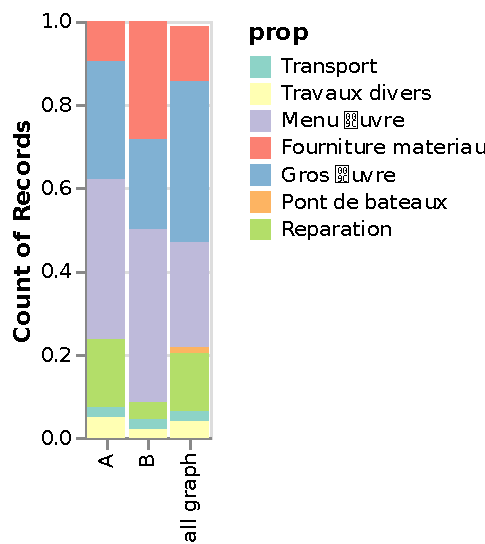
\includegraphics[width=0.2\linewidth]{static/figures/ComBiNet/OriginalPaperFigures/comparisonPlots/type_travail}
    % 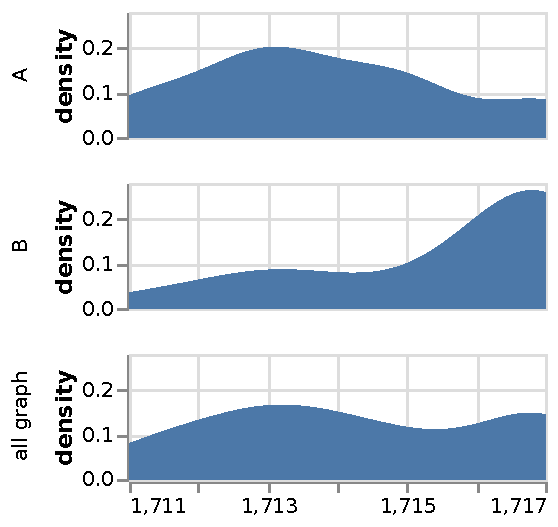
\includegraphics[width=0.2\linewidth]{static/figures/ComBiNet/OriginalPaperFigures/comparisonPlots/date_year}
    % 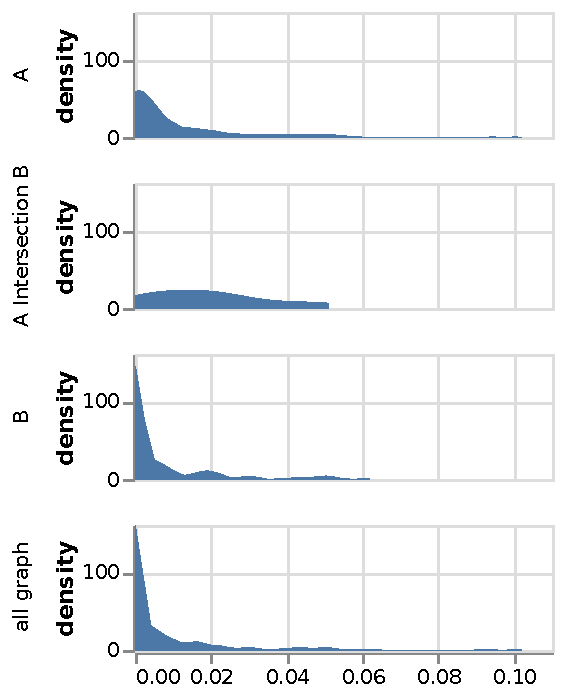
\includegraphics[width=0.2\linewidth]{static/figures/ComBiNet/OriginalPaperFigures/comparisonPlots/Betweeness_Centrality}

    % 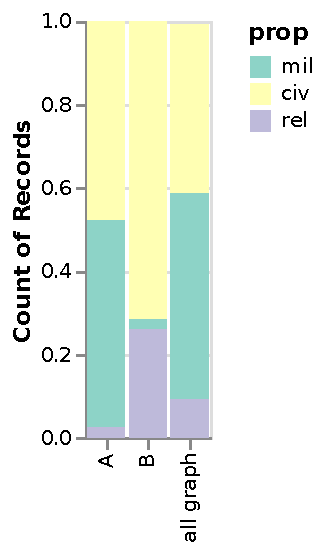
\includegraphics[height=90px]{static/figures/ComBiNet/OriginalPaperFigures/comparisonPlots/type_chantier}
    % % 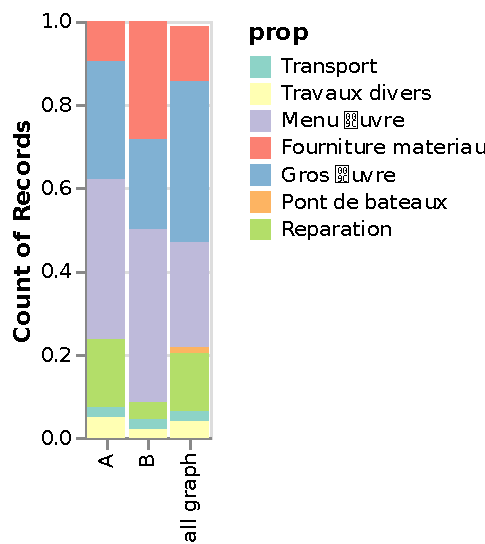
\includegraphics[width=0.2\linewidth]{static/figures/ComBiNet/OriginalPaperFigures/comparisonPlots/type_travail}
    % 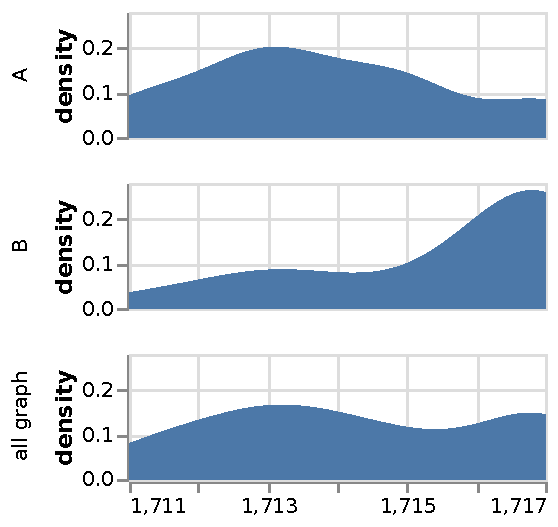
\includegraphics[height=90px]{static/figures/ComBiNet/OriginalPaperFigures/comparisonPlots/date_year}
    % 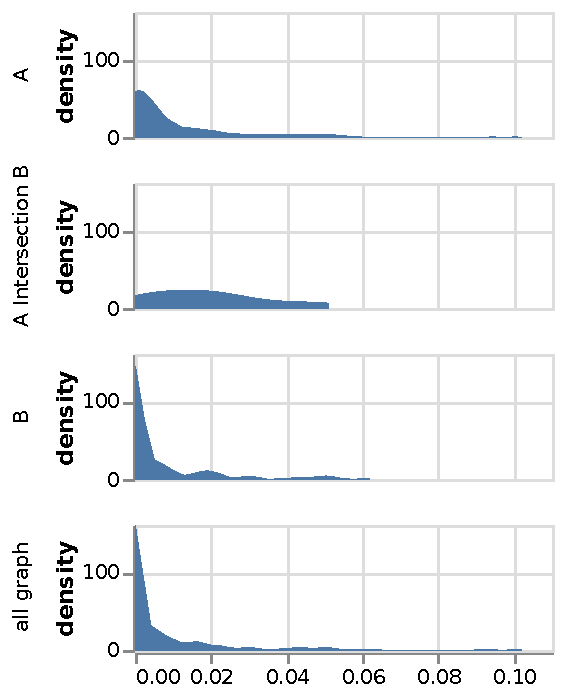
\includegraphics[height=90px]{static/figures/ComBiNet/OriginalPaperFigures/comparisonPlots/Betweeness_Centrality}

    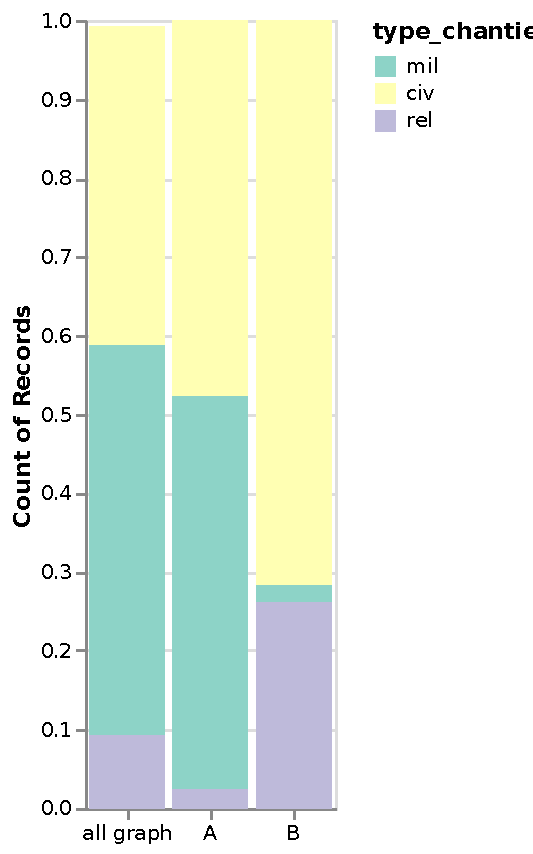
\includegraphics[height=110px]{static/figures/ComBiNet/OriginalPaperFigures/CGF/TurinPlots/type+chantier.pdf}
    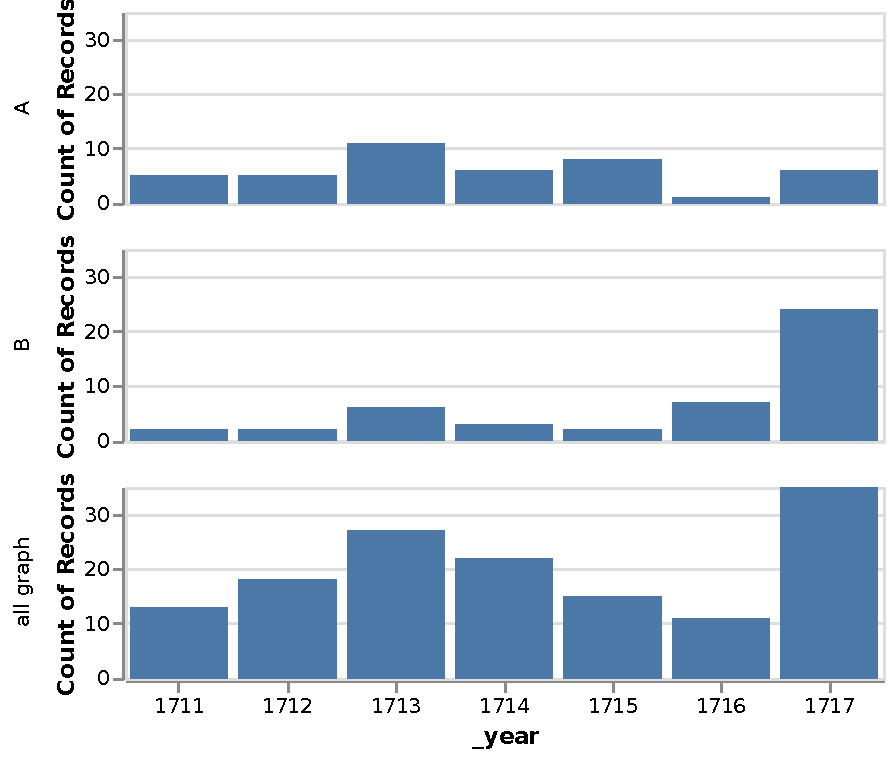
\includegraphics[height=110px]{static/figures/ComBiNet/OriginalPaperFigures/CGF/TurinPlots/time.pdf}
%    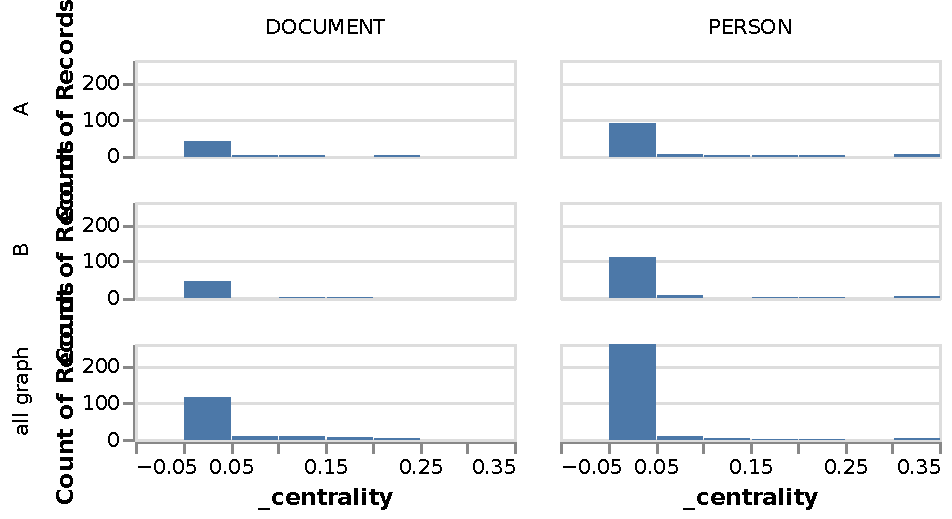
\includegraphics[height=90px]{static/figures/ComBiNet/OriginalPaperFigures/CGF/TurinPlots/centrality.pdf}
    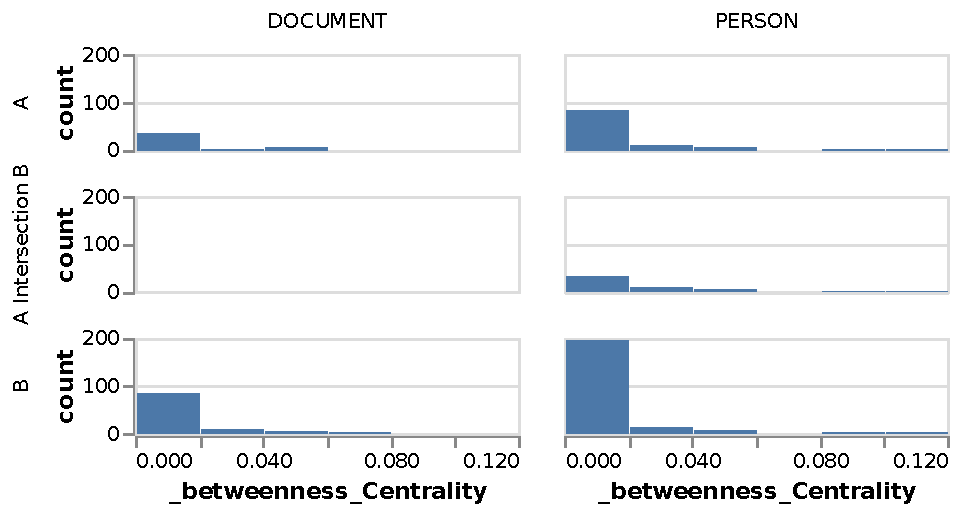
\includegraphics[height=110px]{static/figures/ComBiNet/TorinoCompBC.pdf}

    \caption{Distribution of the type of constructions, the years, and the betweenness centrality for the documents and signatories of Torino (A), Torino surroundings (B), and the whole graph (top).}\label{fig:attributeComparison}
%    \caption{Distribution of two document attributes and one global attribute for the documents and signatories of Torino (A), Torino surroundings (B), and the whole graph. (top).}\label{fig:attributeComparison}
\end{figure}


\subsection{Implementation}

\name is made of three components: a web visual interface, a python server, and a Neo4j\cite{neo4j} graph database instance.
The client interface is written in JavaScript using D3~\cite{d3}, Vega~\cite{satyanarayan2016vega}, and the Trrack library~\cite{cutlerTrrackLibraryProvenanceTracking2020}.
The python server is written in Flask and interacts with the Neo4j instance for query processing before sending the results to the frontend.
We implemented the Cypher parser with the ANTLR parser generator~\cite{parr1995antlr}.
The abstract syntax tree of the Cypher query is used as a representation of the query.
Modifying the query visually updates the tree, which is translated into Cypher in the textual query panel.
Similarly, a manual change in the Cypher query updates the abstract syntax tree which is translated into a visual query.

%\todo{Talk about AST and implementaion}


\section{Use Cases}\label{sec:combinet-usecases}

In this section, I describe how our system has been able to specifically answer questions from three of our collaborators and one other use case.
the tool was mostly operated by the developers working side by side with the collaborators to test the expressiveness of the queries and the value of the results visualizations.
The tool was refined as needed along the way.

% Since usability issues have not been resolved yet, the tool was mostly operated by the developers working side by side with the collaborators to test the expressiveness of the queries and the value of the results visualizations. The tool was refined as needed along the way.

\subsection{Construction sites in Piedmont (\#1)}

One of the main questions of our collaborator was to compare two families which he knew played a big role in the structure of the network: the \textit{Menafoglio} and \textit{Zo} families (question 4 in \autoref{tab:tasks}).
Specifically, he was interested in knowing if there were differences in specialization in the type of contracts and area of work for the core members of these families, and to what extent the two families were collaborating.
Moreover, he was very interested in characterizing the group of people collaborating with both families.

To answer those questions, we first selected the core members of the \textit{Menafoglio family}, by checking the people known by the historian, and their close neighbors.
Looking at the bipartite view (see \autoref{fig:combinet-mena} (a), we can see that the group is pretty dense with people collaborating a lot between them.
Looking at the map, we can clearly see that the family has been mostly active in Piedmont outside of Torino and Torino's close territory.
We also have a first view of the attribute distribution of the persons in the group and their contracts.
\begin{figure}[!ht]
    \centering

     \begin{subfigure}[b]{1\linewidth}
    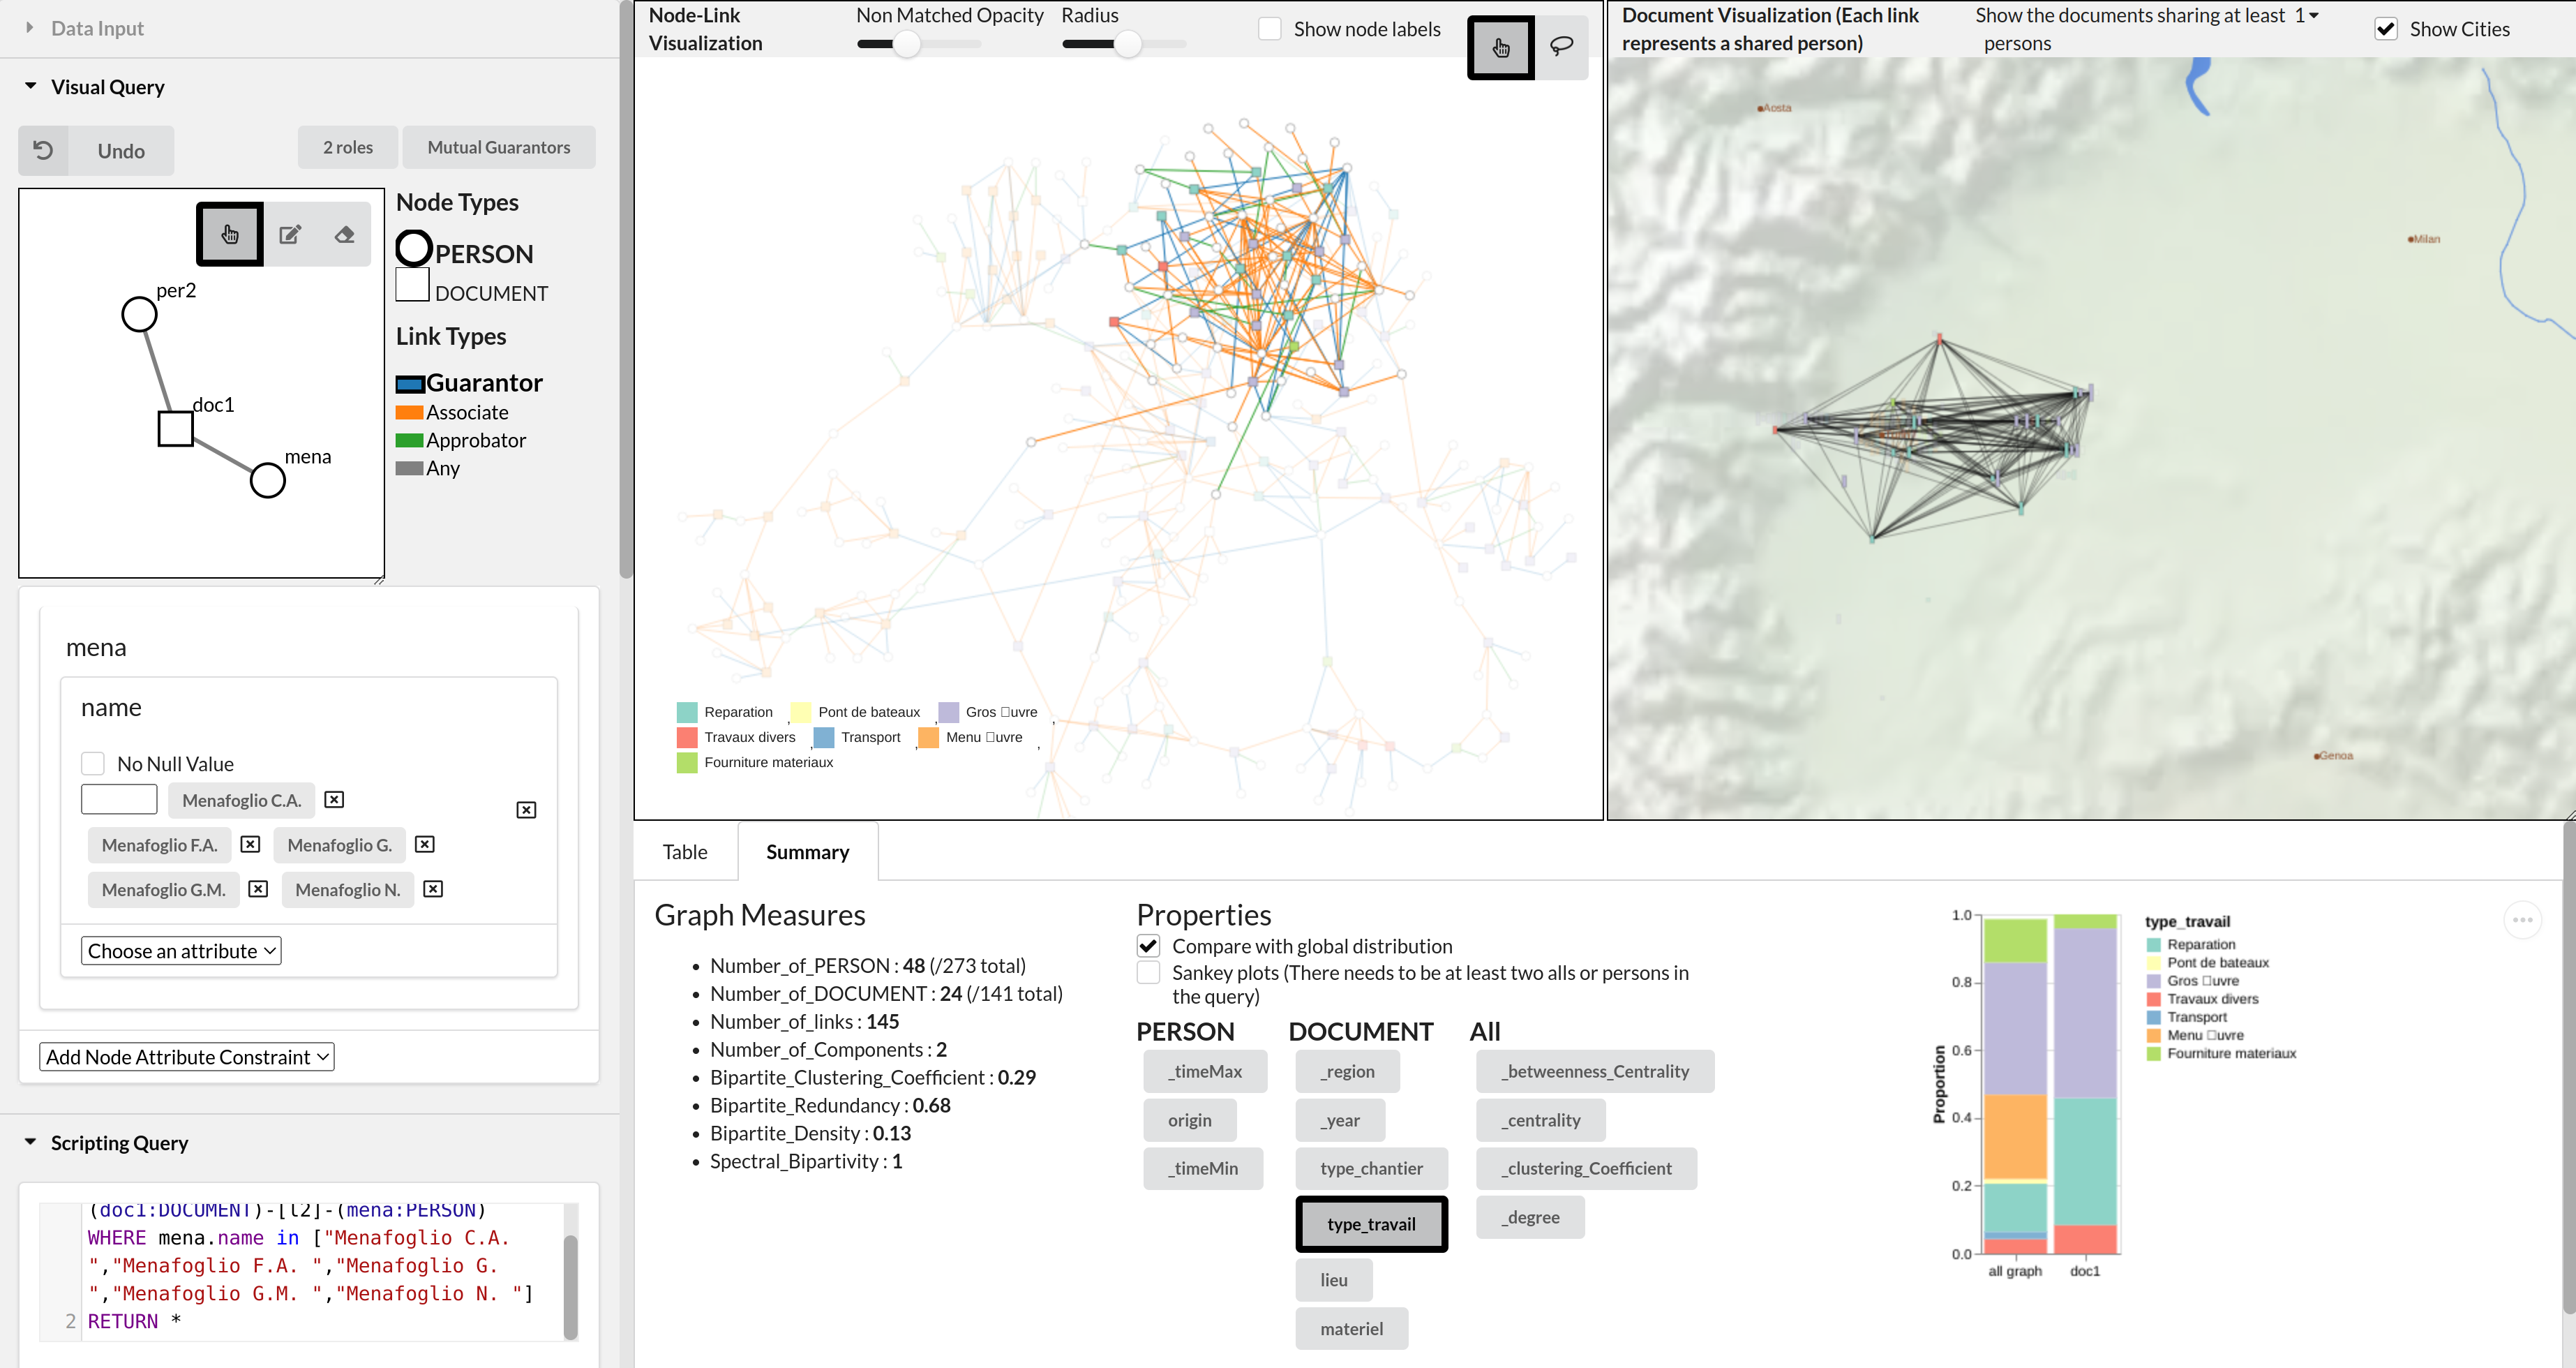
\includegraphics[width=1\linewidth, trim={35cm 37cm 10cm 0}, clip]{static/figures/ComBiNet/OriginalPaperFigures/suppMaterial/menaFamilyResults}
         \caption{}
    \end{subfigure}
    \begin{subfigure}[b]{1\linewidth}
        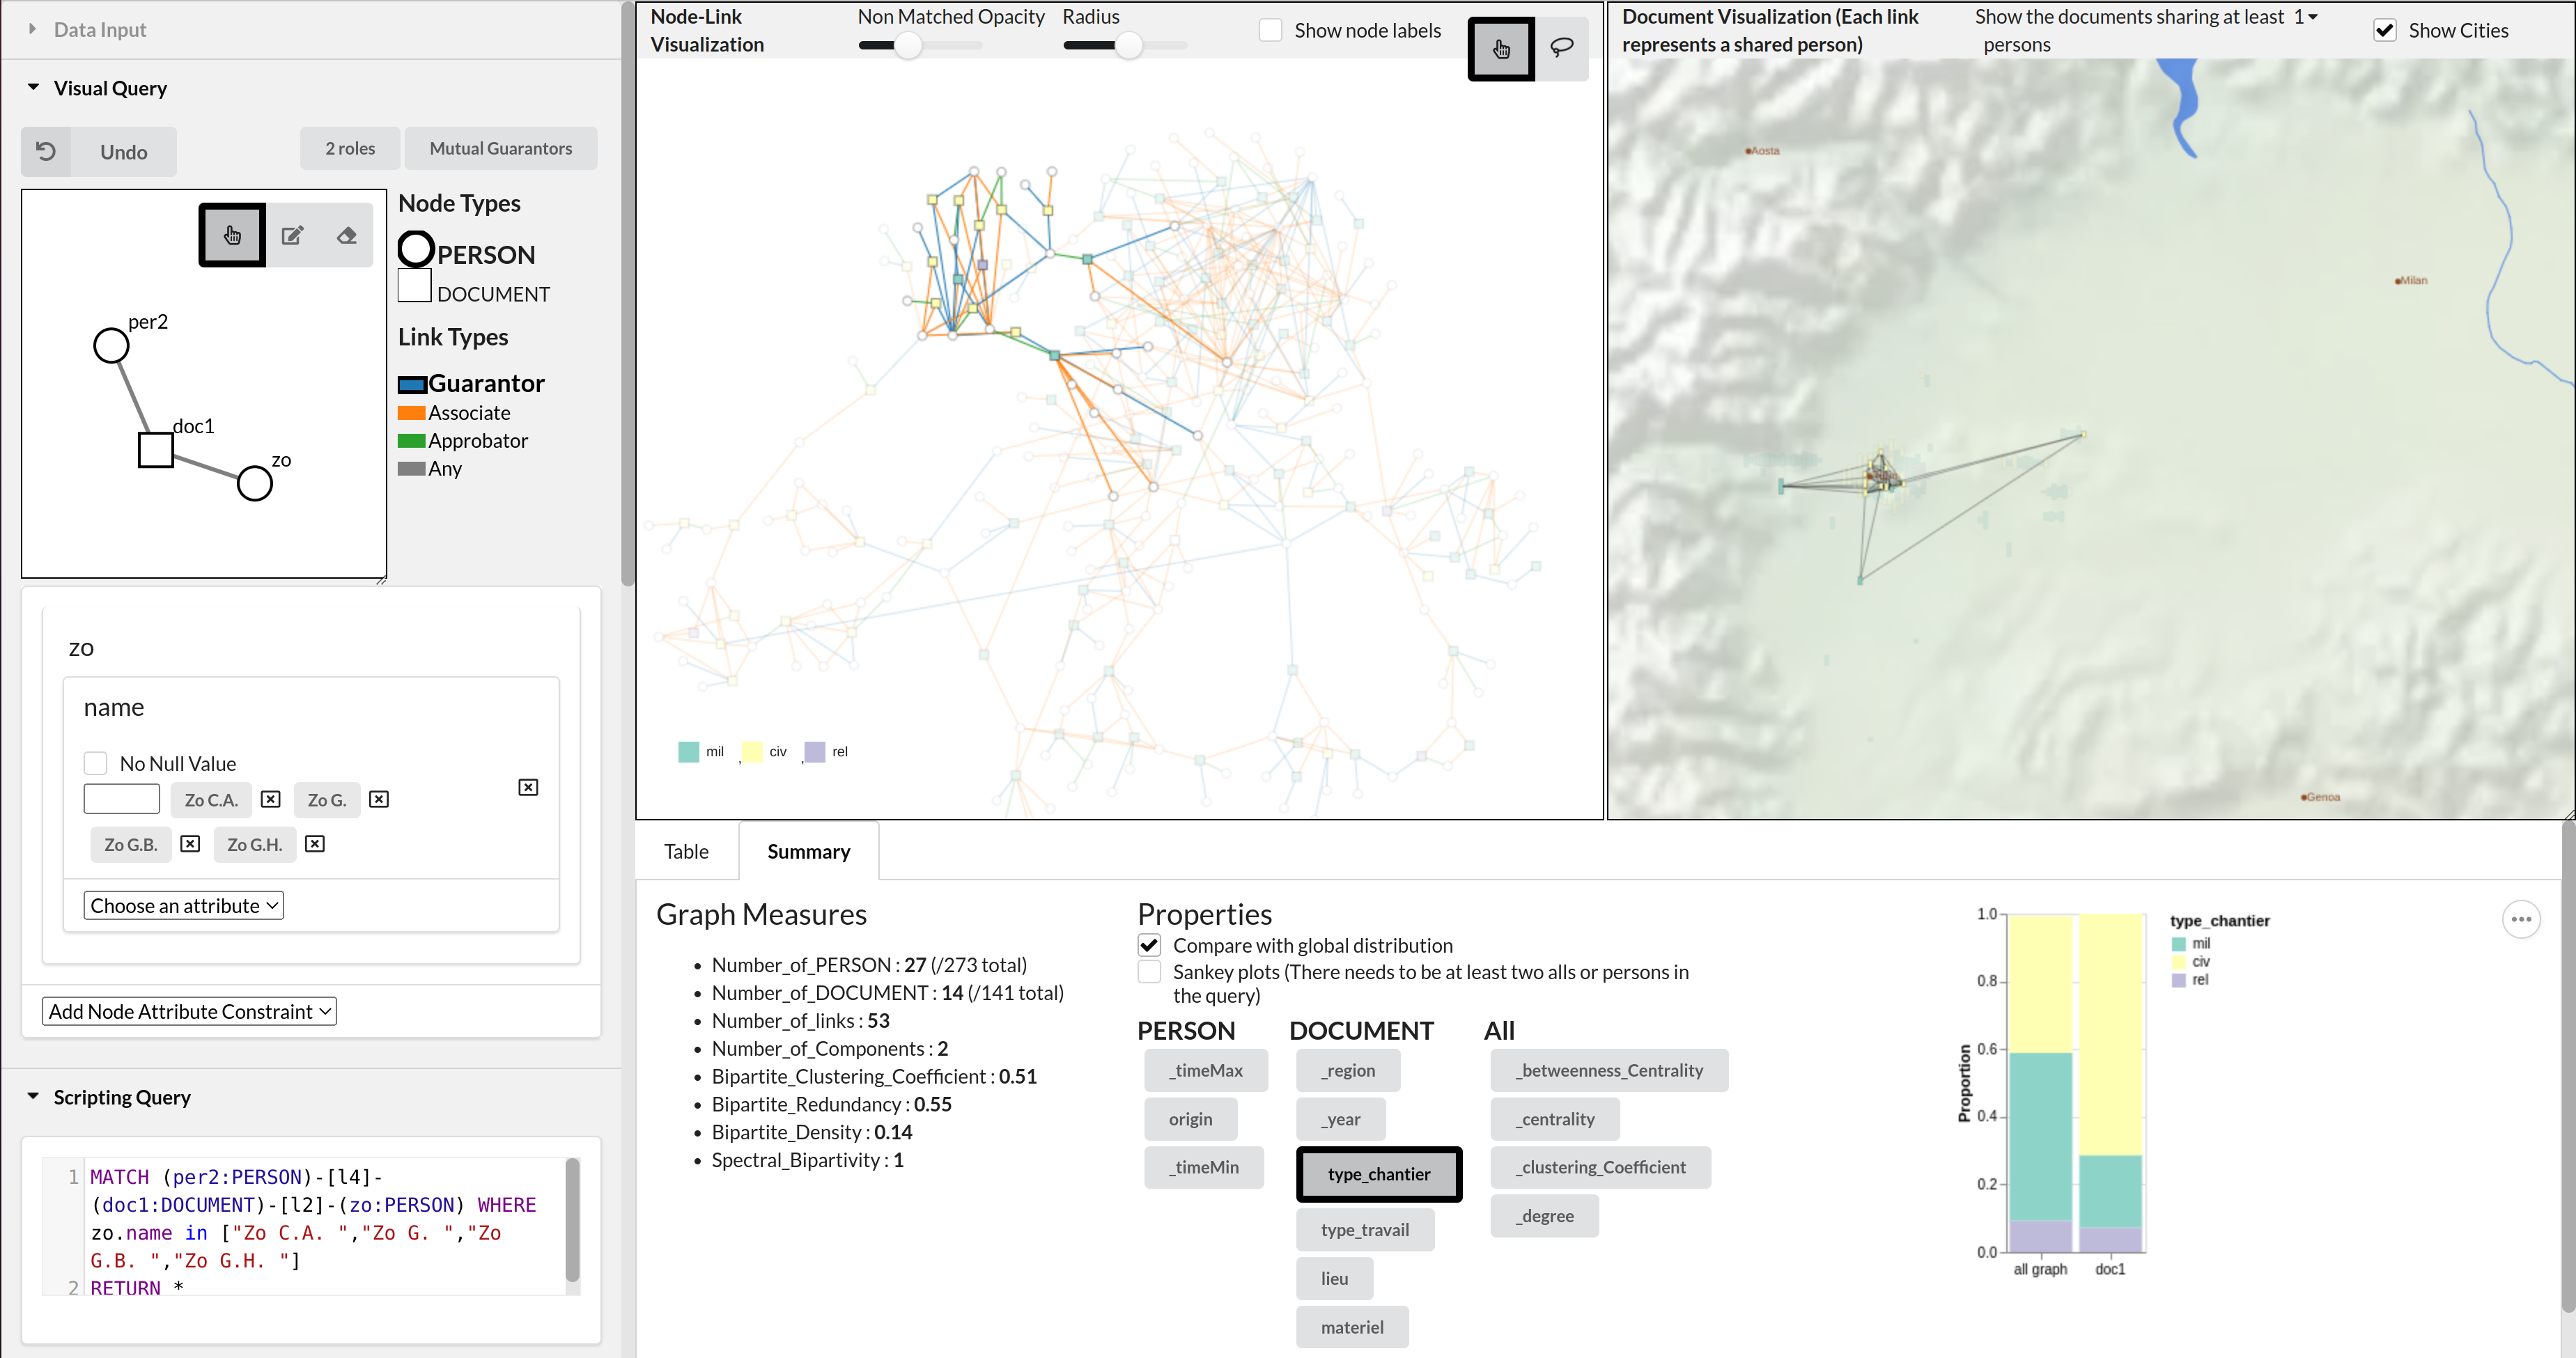
\includegraphics[width=1\linewidth, trim={35cm 37cm 10cm 0}, clip]{static/figures/ComBiNet/OriginalPaperFigures/suppMaterial/ZoFamilyResults}
        \caption{}
    \end{subfigure}

    \caption{Menafoglio (a) and Zo (b) families were retrieved with queries and highlighted in the bipartite node-link and map views.}
    \label{fig:combinet-mena}
\end{figure}
We then do the same query for the Zo family. We keep the same topological filter and replace the name filters with the core members of the Zo family known by the historian. We see on the graph view (Figure 2 of the supplementary material) that the group is smaller and is in a different area in the graph. The map enriched with a selection of the \textit{region} attribute shows that, contrary to the Menafoglio, the Zo family has been more active in Torino and Torino territory (a very close area of the city).
\begin{figure}[!ht]
    \centering
%    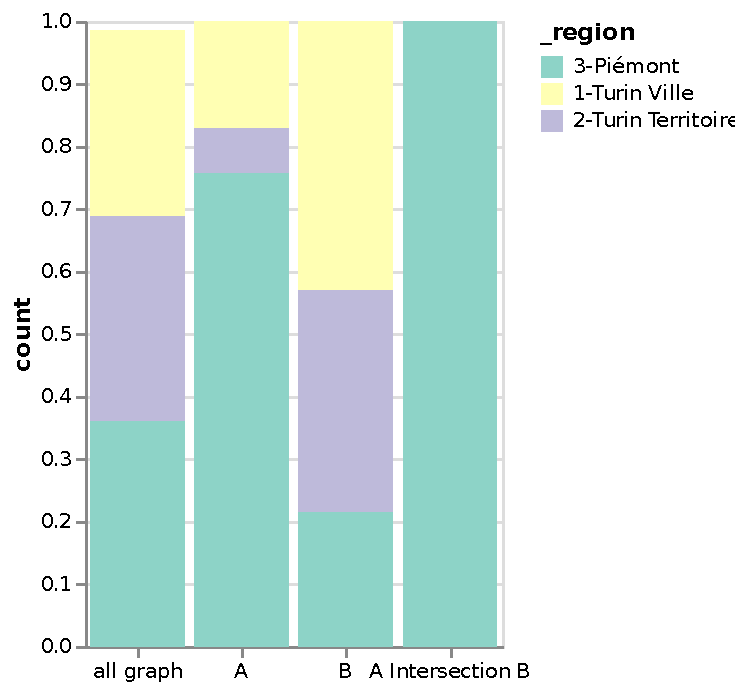
\includegraphics[width=0.3\linewidth]{static/figures/ComBiNet/OriginalPaperFigures/CGF/MenaZoPlots/v2/region.pdf}
%     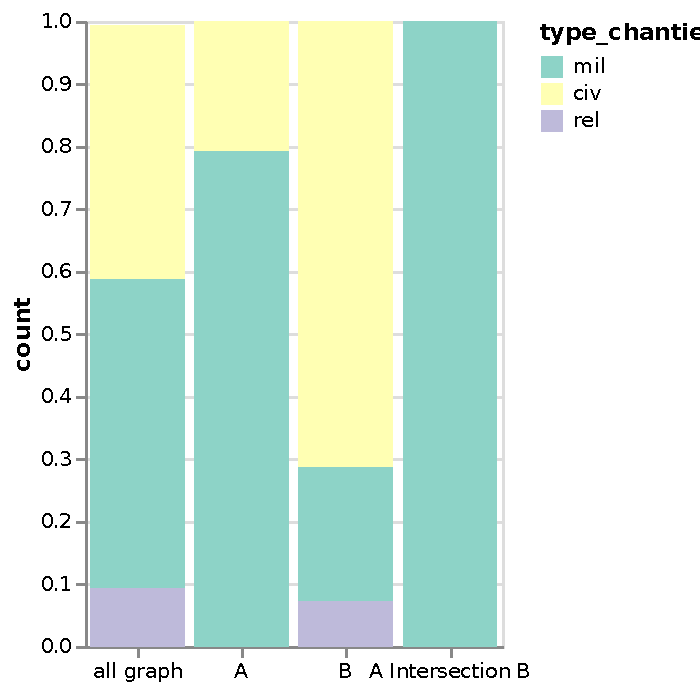
\includegraphics[width=0.3\linewidth]{static/figures/ComBiNet/OriginalPaperFigures/CGF/MenaZoPlots/v2/type-chantier.pdf}
%     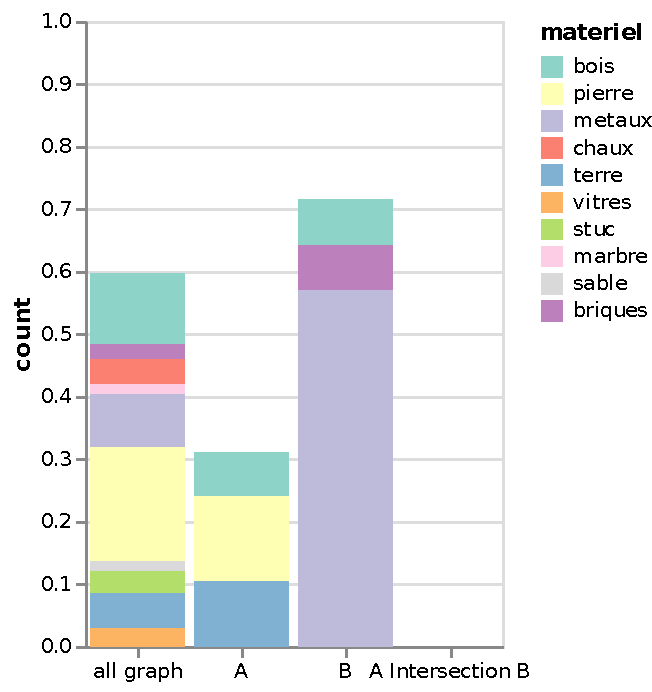
\includegraphics[width=0.3\linewidth]{static/figures/ComBiNet/OriginalPaperFigures/CGF/MenaZoPlots/v2/materiel.pdf}
%     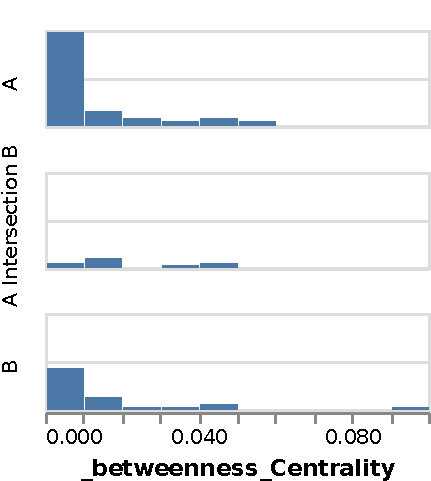
\includegraphics[width=0.35\linewidth]{static/figures/ComBiNet/OriginalPaperFigures/CGF/MenaZoPlots/v2/BC_crop.pdf}
    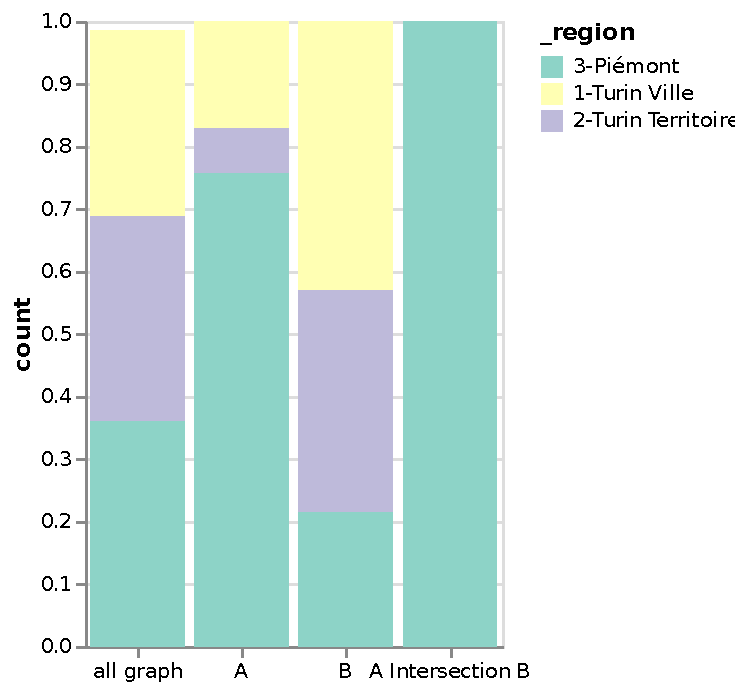
\includegraphics[width=0.34\linewidth]{static/figures/ComBiNet/OriginalPaperFigures/CGF/MenaZoPlots/v2/region.pdf}
     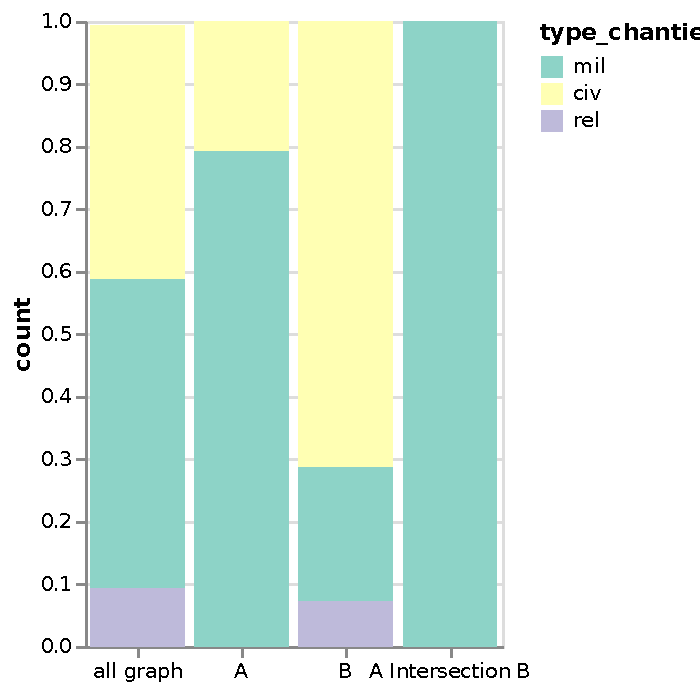
\includegraphics[width=0.34\linewidth]{static/figures/ComBiNet/OriginalPaperFigures/CGF/MenaZoPlots/v2/type-chantier.pdf}
     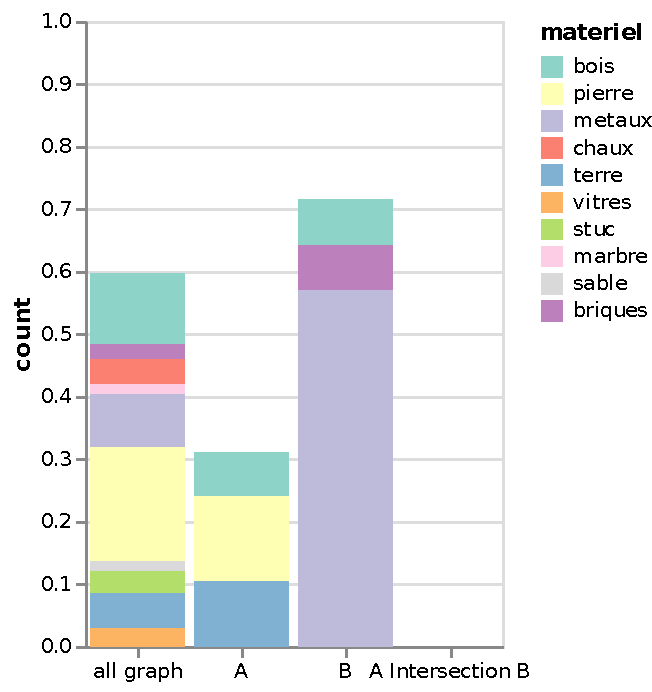
\includegraphics[width=0.34\linewidth]{static/figures/ComBiNet/OriginalPaperFigures/CGF/MenaZoPlots/v2/materiel.pdf}
     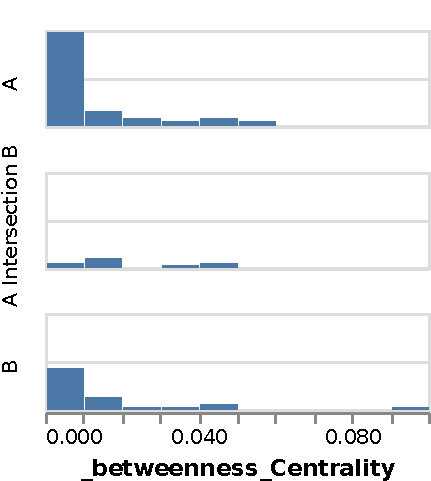
\includegraphics[width=0.34\linewidth]{static/figures/ComBiNet/OriginalPaperFigures/CGF/MenaZoPlots/v2/BC_crop.pdf}

    \caption{Attributes distributions plots between the whole graph, the \textit{Menafoglio} family (A), the \textit{Zo} family (B), and $A\cap B$, for the \textit{region,type\_chantier,  material type.}
    % , and \textit{betweeness centrality}.}
    \label{fig:useCasePascal}}
\end{figure}
The two groups can be compared using the \textit{comparison mode} by selecting the two queries in the provenance tree. This opens the comparison menu to quickly navigate between the visual selection of (A), (B), and the set $A \cap B$ that interests our collaborator. The table showing the graph measures of the two subsets confirms what is shown visually: the Menafoglio group is more populated but less dense than the Zo family.

Our user is then interested in comparing the distribution of several attributes between the two groups. We can clearly see in \autoref{fig:useCasePascal} (top right) that the Menafoglio family is more specialized in military (\textit{mil}) sites, while the Zo family is doing more civil (\textit{civ}) constructions. This is confirmed by the \textit{material} distribution that shows that the contracts of the Menafoglio are often using stones, whereas it is never the case for Zo contracts.
Finally, the persons collaborating in the two groups have a betweenness centrality higher on average (bottom right, middle chart).
This makes sense as they act as bridges linking the two families.
% Moreover, we can see in detail the difference in the region of contracts of the two families.





% \begin{figure*}
%     \centering

%     \begin{overpic}[width=\linewidth]{static/figures/ComBiNet/OriginalPaperFigures/useCase01/queryAndComparePascal}

%      \put(30,14){\small Comparison}
%     %  \put(25, 22){\circled{\large A}}
%     \put(25, 4){\circled{\large I}}
%      \put(40, 4){\circled{\large II}}
%     \end{overpic}

%     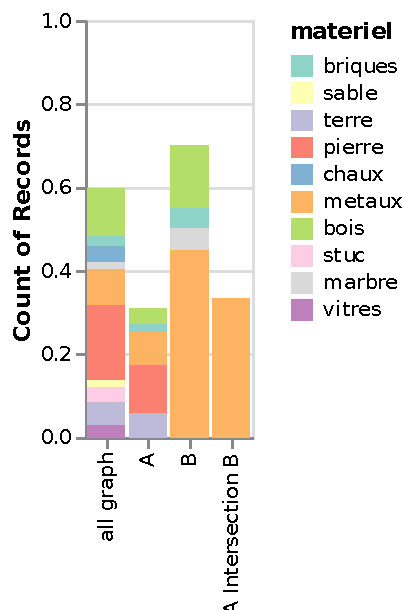
\includegraphics[height=120px]{static/figures/ComBiNet/OriginalPaperFigures/useCase01/attributes/materiel.pdf}
%     %  \includegraphics[width=0.2\linewidth]{static/figures/ComBiNet/OriginalPaperFigures/useCase01/attributes/region.pdf}
%      \includegraphics[height=120px]{static/figures/ComBiNet/OriginalPaperFigures/useCase01/attributes/type_chantier.pdf}
%      \includegraphics[height=120px]{static/figures/ComBiNet/OriginalPaperFigures/useCase01/attributes/type_travail.pdf}
%      \includegraphics[height=120px]{static/figures/ComBiNet/OriginalPaperFigures/useCase01/attributes/betweenness.pdf}

%     \caption{Comparison of the two group of interests for use case \pascal. (I) shows the two queries the user created to select the two groups of interest. (II) presents \name in comparison mode, with the intersection of (A) and (B) selected. The table shows the structural difference of the two groups, while the two graph views highlight the persons who collaborated between the two groups, who are of interest for our collaborator. The user selected the \textit{region} attribute, creating a plot showing that the Menafoglio and Zo families are working respectfully more in Piemont and Torino, while their collaboration has no strong associated region.}  \label{fig:useCasePascal}
% \end{figure*}

%\vspace{-1mm}
\subsection{French Genealogy (\#2)}

We describe how \name allowed us to answer an important question of the use case \nicole: to detect the largest migrations across several generations, in which areas, and at what time they occurred (question 9 in \autoref{tab:tasks}).
The map view shows at a glance (\autoref{fig:useCaseNicoleMap}) that the majority of events have taken place in three specific regions: west (Britany), mid-north (Paris), and mid-south (Limousin).

\begin{figure}[!ht]
    \centering
    \includegraphics[trim={82cmcm 30cm 0 0},clip,width=0.8\textwidth]{static/figures/ComBiNet/OriginalPaperFigures/suppMaterial/FrenchGenealogy}
    \caption{Map of the migrations in France which occurred across several generations.}\label{fig:useCaseNicoleMap}
\end{figure}

To find patterns of migrations within families, we first make a query representing a simple family by linking a person node to a birth event, connected to the parents using a link of \textit{father} or \textit{mother} type. We repeat the process to the new parent node to add another generation. Finally, we connect the latest generation child with a death event, to have another date and location to compare to (see \autoref{fig:UseCaseNicoleQ}). This query returns every person with their parents and grandparents, along with their respective birth and death data for the latest person. We also create a constraint on the \textit{department} attribute on the documents to only retrieve the events that have a non-null associated location. This request returns a subgraph of 64 persons and 88 documents. The user can now select the \textit{department} attribute to create a Sankey diagram that shows the change of departments across the different generations of families. \autoref{fig:UseCaseNicoleS} shows that the majority of families are from \textit{Haute-Vienne} (which can easily be confirmed by checking the map), and do not move much across generations. Our collaborator however detected interesting patterns of people moving from the department \textit{Creuse} to \textit{Haute-Vienne} across two generations. She refined the query by adding an attribute filter on this specific department using a widget. The table view then showed her who these migrants were and when it occurred. The bipartite visualization panel allowed exploring more in-depth this specific group of people. %, with their close neighbors.


% We now can use the Sankey visualization of the \textit{department} attribute to see if there is interesting patterns of migration.
\begin{figure}[!ht]
    \centering
    % \begin{subfigure}{0.49\linewidth}
    % \includegraphics[width=\textwidth]{static/figures/ComBiNet/OriginalPaperFigures/useCase02/queryParents3gen.png}
    % \caption{Visual query to find all 3-generation families (documents without department have been filtered out)}
    % \label{fig:UseCaseNicoleQ}
    % \end{subfigure}
    % % \includegraphics[width=0.4\linewidth]{static/figures/ComBiNet/OriginalPaperFigures/useCase02/armorConstraint.png}
    % \begin{subfigure}{0.49\linewidth}
    % \includegraphics[width=\textwidth]{static/figures/ComBiNet/OriginalPaperFigures/useCase02/sankey3genDep.pdf}
    % \caption{Sankey diagram showing the birthplace of people across generations and the death place}
    % \label{fig:UseCaseNicoleS}
    % \end{subfigure}

    \begin{subfigure}[b]{0.4\linewidth}
    \includegraphics[width=\textwidth]{static/figures/ComBiNet/OriginalPaperFigures/CGF/frenchGenealogy/migrationQuery.png}
    \caption{Visual query to find all 3-generation families %(only documents mentioning a department are shown)
    }
    \label{fig:UseCaseNicoleQ}
    \end{subfigure}
    % \includegraphics[width=0.4\linewidth]{static/figures/ComBiNet/OriginalPaperFigures/useCase02/armorConstraint.png}
    \begin{subfigure}[b]{0.59\linewidth}
    \includegraphics[width=\textwidth]{static/figures/ComBiNet/OriginalPaperFigures/CGF/frenchGenealogy/migration3.pdf}
    \caption{Sankey diagram showing the birth and death places of people across generations}
    \label{fig:UseCaseNicoleS}
    \end{subfigure}

    \caption{Migrations across departments over three generations}\label{fig:useCaseNicole}
\end{figure}

Afterward, we answered question 9 (\autoref{tab:tasks}), \ie is there a significant difference in the migrations between the 18th and 19th centuries.
She thought people started moving in the 19th century and wanted to confirm it.
To answer this, we first created a query to retrieve the people with birth and death certificates from a specified department.
We then applied a time filter on the death certificate node, first for the 18th century and then the 19th century, compared the two query results using the comparison mode, and looked side by side the Sankey graphs related to \textit{departments} (\autoref{fig:useCaseNicole2}).
We can clearly see that people do not move at all in the 18th century, while in the 19th century even if the majority of people stay in the same place from their birth to their death, more than half moved.
It thus confirms the hypothesis of our collaborator.

\begin{figure}[!ht]
    \centering
    % \begin{subfigure}{0.49\linewidth}
    % \includegraphics[width=\textwidth]{static/figures/ComBiNet/OriginalPaperFigures/useCase02/sankeyDep18c.pdf}
    % \caption{18th century}
    % \end{subfigure}
    % \begin{subfigure}{0.49\linewidth}
    % \includegraphics[width=\textwidth]{static/figures/ComBiNet/OriginalPaperFigures/useCase02/sankeyDep19c.pdf}
    % \caption{19th century}
    % \end{subfigure}

    \begin{subfigure}{0.49\linewidth}
    \includegraphics[width=\textwidth]{static/figures/ComBiNet/OriginalPaperFigures/CGF/frenchGenealogy/migration_18.pdf}
    %\caption{18th century}
    \end{subfigure}
    \begin{subfigure}{0.49\linewidth}
    \includegraphics[width=\textwidth]{static/figures/ComBiNet/OriginalPaperFigures/CGF/frenchGenealogy/migration_19.pdf}
    %\caption{19th century}
    \end{subfigure}

    \caption{Sankey diagrams showing the migration of people in the 18th and 19th centuries, extracted from their birth and death places.}\label{fig:useCaseNicole2}
\end{figure}


\subsection{Marriage acts in Buenos Aires (\#3)}\label{subsec:usecase-BA}
%6659 PERSONS. 1381 MARRIAGE_ACTS.
I present in this subsection how \combinet has been used to detect erroneous encoding during the annotation process of the marriage acts of our collaboration \zacarias.
The 1381 documents mention 6659 individuals, who can have the same name, especially between fathers and sons in this period and region as specified by our collaborator.
During the annotation process, the historian and his collaborators gave identifiers to the persons mentioned in the documents---which is typically part of the annotation procedure.
However, in the case of homonyms, it can be hard to know if some mentions between different documents refer to the same or different persons.
Historians cross the information contained in the different documents to disambiguate the persons\cite{winchesterLinkageHistoricalRecords1970}, but errors can easily be made, \ie giving the same identifier to different persons or giving different identifiers to the same person.
I used \combinet in collaboration with researchers of this project to detect erroneous patterns and help them refine their encoded data.
%For this, we created a query to detect persons mentioned in two acts either as \textit{husband}, \textit{wife}, or \textit{witness} with a time difference of 70 years or more.
For this, we can find the persons mentioned in two acts either as \textit{husband}, \textit{wife}, or \textit{witness} with a time difference of 70 years or more.
Such person nodes in the network represent with almost full certainty two different persons who lived in different generations.
We constructed a request to find this pattern with the visual query view and added the time constraint between the two marriage acts with the Cypher textual input.
\begin{figure}[!ht]
    \centering
    \includegraphics[width=\linewidth]{static/figures/ComBiNet/BuenosAires_correction}
    \caption{\name used to request persons appearing as husband, wife, or witness in two marriages that occurred 70 years apart or more.}\label{fig:combinet-BuenosAires-correction}
\end{figure}
%returning this pattern visually and added the time constraint between the two marriage acts with the Cypher view.
\autoref{fig:combinet-BuenosAires-correction} shows the visual query constructed (left), the bipartite view with the persons and documents matching the query highlighted (middle), and the table listing all the documents having mentions of people with erroneous identifiers (bottom right).
%The query returned 29 persons found in this pattern.
The table permits to browse through all person nodes (29 have been found) that correspond in fact to more than one person and to the documents which contain the wrongly given identifiers.
Using the exporting capabilities, our collaborator has exported the occurrence table indicating the pairs of documents (with their identifiers) mentioning two different persons who have been given the same identifier.
Using this table, he has been able to rapidly correct those errors in his annotation framework.




% 54 occurence, 71 documents, 29 persons
%MATCH (mar2:MARRIAGE_ACT)-[l3:HUSBAND|WIFE|WITNESS]-(per1:PERSON)-[l:WIFE|HUSBAND|WITNESS]-(mar1:MARRIAGE_ACT) where mar1._year - mar2._year > 70 RETURN *
%6659 PERSONS. 1381 MARRIAGE_ACTS




\subsection{Sociology thesis in France}

I describe in this fourth use case how \name can be used to answer questions about the thesis in France between 2016 and 2022.
Indeed, some sociological datasets made of documents can also be well modeled as \modelplural, like thesis dissertations: a thesis is a document with specific attributes such as the subject, the doctoral school, the domain, the university, and the date of defense, and mention several peoples who are socially connected through the thesis defense with different roles: author (\textit{auteur} in french), director(s) (\textit{directeur}), reviewers (\textit{rapporteur}), and jury president (\textit{président de jury}).
%We discussed with sociologists who were interested in this type of data for explorations purposes.
We present here an exploration of the data by ourselves using \name.
A first look at the graph measures tells us that 896 theses have been defended in sociology in France between 2016 and 2021 in France, with 2453 persons included in the defenses (see \autoref{fig:combinet-thesis-exploration} bottom).
The bipartite node-link view shows us an overview of the network but is hard to parse due to the network's size.
Zoom actions though allow us to center the view on specific parts of the network.
The map view reveals that theses has been defended all around France, even though the majority are defended in Paris.
\begin{figure}[!ht]
    \centering
    \includegraphics[width=0.8\textwidth]{static/figures/ComBiNet/Thesis-first-exploration}
    \caption{\name used for exploring theses of sociology defended in France between 2016 and 2021. The bipartite and map views show an overview of two visions of the network. The user selects the \textit{region} attribute, showing the geographical distribution of the defended thesis.}\label{fig:combinet-thesis-exploration}
\end{figure}
This is confirmed by a look at the distribution of the cities (\autoref{fig:combinet-thesis-exploration} bottom right): around half of the defenses are in Paris, compared to the rest of the country which is more or less homogeneous.
By setting the threshold to link creation to one (meaning that a link is created between two documents if they mention at least one common person), a lot of links are created as seen in \autoref{fig:combinet-thesis-exploration} (right).
It means that a lot of thesis defenses include reviewers and juries from different cities.

Let's now try to answer an interesting question: ``Do reviewers and jury presidents often ask thesis directors to be reviewers and jury presidents in their turn for another thesis where they are directors ?''.
For this, we can construct a visual query representing this pattern by creating two person nodes and two document nodes, and by connecting them with two president links and two reviewers or jury director links in a symmetrical way, as shown in \autoref{fig:combinet-thesis-query} (right).
The occurrence table tells us that this pattern has been found 76 times in the network, meaning that this is a recurrent behavior.
We are now interested in characterizing the thesis occurring in this pattern, by their regions.
We can look at the \textit{city} attribute distribution for this thesis by selecting it in the attribute view as shown in \autoref{fig:combinet-thesis-query} (bottom right).
We can first see on the map that this pattern occurs mainly in the biggest cities of the country.
By selecting the Sankey view option, we can investigate if this pattern occurs between thesis defended in different regions or if it occurs mainly in the same ones.
We learn that it depends mainly on the regions: in Bourgogne-Fanche-Comté 26 out of 29 theses are connected with the thesis of another region.
On contrary, in \textit{Occitanie} it is the case for only 4 out of 17.
On average, we can see that this pattern occurs a lot for theses of the same region.
In Ile-de-France, it is the case for around half of the thesis (28/50).
This exploratory analysis shows that \name can be used to explore and gain insight into this type of sociological dataset.

\begin{figure}[!ht]
    \centering
    \includegraphics[width=0.8\textwidth]{static/figures/ComBiNet/Thesis-query01-and-results}
    \caption{Sociology thesis dataset explored with \name. The user constructed a visual query to see if there are symmetrical relationships between thesis directors and reviewers (or jury directors). The \textit{region} attribute is selected with the Sankey option, letting the user see if there are correlations between the regions of the thesis found in this pattern.  }\label{fig:combinet-thesis-query}
\end{figure}

\section{Formative Usability Study}\label{sec:combinet-usability}

%\subsection{Procedure}

% After showing our tool can be used to answer socio-historical questions,
I performed a formative usability study with two historians and one expert in visualization.
I had 3 meetings with each and gave them control of the tool to see if they could use it to explore their data---the visualization expert used the interface with the dataset of construction contracts \pascal---and perform queries and comparisons.
At the first meeting, I explained to them the panels of the system and each feature.
During each session, they were free to explore the data as they wanted.
If they were stuck using one feature, I helped them by explaining how to use it.
If they seemed to not know what to do next, I asked them to answer a specific question on the data (for example ``can you find the persons who collaborated in more than two contracts between 1711 and 1714 in Torino'').
At each meeting, I asked them to speak aloud, commenting on their aims and actions.
At the end of each session, they reported their general feedback, what they did not like or understand, and what other features they would like to have to explore their data.

I improved the system and made the changes asked by the users before setting up new appointments.
This usability study led to the redesign of some core features, like the activation of the comparison mode which is now started by first marking the state nodes in the provenance tree.
It also led to the implementation of new features, such as the person and document tables (which are updated after each query), the persistent selection of nodes across the two views and the tables, and the undo feature for visual queries.
% The list of all feedback and modifications are shown in the supplementary material.
At the final meetings, the three users were able to perform exploration, queries, and comparisons to answer socio-historical questions by themselves.


\subsection{Feedback}

All three users liked the table views and were exploiting them to study in depth who were the person and documents found in their specific queries.
Both historians liked the Sankey diagram of the attributes, allowing them to see the evolution of distributions and answering several of their questions.
Our collaborator of the use case \nicole was making sense of it by linking the migration patterns she was seeing in the Sankey diagram with specific persons of the dataset she knew in depth.
She was also curious about other migration patterns she was not aware of and wanted to know who these persons were, the system allowing her to select them and follow a deeper exploration.
One other historian outside of our direct collaborators liked the overlay of node attributes on the bipartite and map views, and the distribution plots. She said: ``With this data model, even if historians realize the structure of their network does not allow them to answer their research questions, they can still visualize and compare attributes of documents and persons with this interface, which is always useful in quantitative history''.

% [jdf] You don't mention theses capabilities in the paper
% Both liked the export capabilities of the system to collect results in CSV or JSON format, as well as the charts in SVG, for inclusion in their publications or for processing with other tools.



\iffalse
\section{Discussion}

Useful to social scientists provide a good trade-off between expressive power and simplicity compared to alternatives, either not expressive enough or too complex.

Compared to other systems:
\textbf{Jigsaw}: close on many aspects, also relies on a stable data model, but more expressive using attributes and roles. Yet, we do not handle general named entities that seem less important than for intelligence analysis; they can sometimes be emulated with attributes.

We applied it to other projects, such as research administration: publication and contracts visualization, and exploration.


\textbf{VERTIGo}: similar for queries, but VERTIGo can adapt to any data model, does not prescribe a data model, and handles attributes.

We want to distribute \name as an open-source tool and facilitate its use.

Still needs the help of a programmer to import data. Other systems, such as Gephi, provide plugins for that.

\jdf{Maybe} We need to improve the usability, most of the use cases have been done with the help of the authors.


Possible discussion points :
- Hard to evaluate
- No dynamic visualization
- A bit hard to do query on the orders of events
- Dirty data
\fi

\section{Discussion}

% We discuss here several points of potential limitations.
I discuss in this section several points of potential limitation for the system.

\noindent\textbf{Query Expressiveness.}
The visual query system currently allows finding occurrences of attributed subgraphs, with potential union operations on constraints (links and node attribute values can be set at one value or as a set of values). Being able to express attribute constraints (other than for labels and ids) and unions is new compared to other visual graph query systems.
More complex constraints are then expressible using the Cypher editor, such as dependent constraints, e.g., if one node attribute value has to be greater or lower than another attribute value.
The visual query system could be extended by introducing more complex time constraints capabilities, such as in~\cite{monroe2012exploring}.

\noindent\textbf{Network Modeling}
In \autoref{ch:hsna-process-and-network-modeling}, I claimed that \va interfaces for \hsna should not only focus on answering high-level analysis questions but also support social historians in their annotation (step 3) and modeling process (step 4).
I showed that \combinet can be used to reflect on the annotations and detect erroneous patterns (precisely in \autoref{subsec:usecase-BA}.), leveraging data modeled as \modelplural.
Concerning the modeling step, \modelplural model the sources in all their complexity, and analysts may want to project the network to have a specific vision of the data to answer a precise question.
\combinet allows focusing on specific parts of the network (one type of role, the time, the locations, or specific attributes) with the help of filters, which return subgraphs highlighting certain aspects of the data.
However, it does not allow to do more complex projections---such as representing only the persons in a projected network---in part due to the limitations of Neo4j\cite{neo4j}.

\noindent\textbf{Scalability.} We assess the scalability in network size (number of nodes and links) concerning the cluttering and readability of the network visualizations. Our biggest dataset from \zacarias\ comprises 7212 nodes (4886 persons and 2326 events) and 7790 links, after splitting the documents into birth and marriage event nodes. The system allows the exploration of networks of this size with a decent frame rate.
% Large networks are usually hard to read due to edge crossings~\cite{shneiderman2006network}.
\name allows navigating relatively large sparse graphs (thousands of nodes) with the node-link visualization using zoom \& pan and filtering with the query system. It lets users focus on subsets of the data, one or two at a time.

\noindent\textbf{Generalizibility.} The system has been designed specifically for \modelplural, which models well a diversity of historical sources we encountered via our collaborations: marriage acts, birth/death certificates, construction/work contracts, census, and migrations forms.
Moreover, \model can also be used to model other similar data types, such as scientific publications or thesis data.
However, other kinds of historical textual data exist where documents can mention each other, such as in private letters for example.
The model and interface would need to be slightly modified to take into account document-to-document links for these datasets.
Bipartite networks are also used in various other disciplines, such as biology~\cite{klamt2009hypergraphs} and chemistry~\cite{konstantinovaApplicationHypergraphTheory2001}. \name could be extended to these other application domains, in particular by modifying the map view to show other location data related to the entities of the network, or removing it altogether if it makes no sense for a particular domain.

% \noindent\textbf{Dynamic representation.} The current system allows to explore the temporal aspect of the data by letting users select a color scale which encodes the time, or by filtering the graph according to a time constraint using the query features. Other layouts taking into account the time could be implemented in the future. The visual query system could also be extended by introducing more complex time constraints capabilities, such as in~\cite{monroe2012exploring}.

% \textbf{Visual and textual queries} As visual queries systems can become overbloated and difficult to use as the power of expression increases, we decided to keep our query system easy to use, with the possibility of refining queries textually.

%\vspace{-1mm}
\section{Conclusion and Future Work}

I presented in this chapter \name, a \va system for exploring social networks modeled from historical textual sources, primarily aimed at social historians.
It relies on modeling documents as bipartite, multivariate, dynamic, geolocated social networks where persons are linked to documents or events using typed links that express roles.
% We have successfully applied our data model to a wide variety of historical, sociological, genealogical datasets, and publication data.
With this data model, \name let historians explore a concrete representation of their annotated documents (\ie the model expresses the \emph{reality} of the documents, without the use of projections or distortions) with \emph{traceability} to the original sources and \emph{simplicity}.
Historians can hence reflect on their encoding process (step 3 of the \hsna workflow as described in \autoref{ch:hsna-process-and-network-modeling}) and answer their socio-historical questions using 1) dynamic queries on the network structure and attributes to highlight groups of interests (step 4 of the \hsna) or erroneous patterns and 2) visual comparisons to contrast selected groups according to their structure, location, time, or any other attribute.
% \name supports dynamic queries that are translated in textual queries in the Cypher language, providing a mixed modality to query data.
The results can be visualized as a bipartite node-link diagram, a geographical map, graph measures, and distributions of values for the attributes.
I have shown that complex explorations and analyses were easy to perform, and validated our approach by first describing four use cases among several other projects we are collaborating with and by performing a formative usability study showing that after many improvements the system is usable by social scientists.
%Our collaborations with social scientists revealed that the process of modeling historical sources into an analyzable network is not easy.
% Several weeks of discussion led to the decision to model their data as \model which allows to have a representation of the original documents while modeling well the social relationships mentioned in the sources. It
%Modeling their data as \model allows social scientists to have a common representation to both cleanup and analyze their data.

By specifying a unifying data model and novel high-level visual and interactive mechanisms for comparing topology, attributes, and time, social scientists were able to correct their data more easily with exploration and querying error-induced patterns.
Thanks to the document-centered model, it was easy for them to trace back the errors and inconsistencies to the sources for corrections.
With the same representation, they were able to operate explorations and analyses using easy-to-use interactions implemented in \name such as coordinated views, visual querying, and comparison.
Using these mechanisms, social scientists performed visual exploratory analyses of their network based on topological and attribute descriptions and comparisons of subgroups of interests---between them or the overall network.
This methodology allows them to either ground or refute their hypotheses in network measures and attribute distributions, or to generate new ones from new insight revealed thanks to the exploratory and interaction mechanisms.

We believe \name leads the way toward a new generation of highly interactive exploration tools applicable to wrangle and analyze a wide variety of real social networks modeled from textual sources, with a focus on the \emph{reality} of the documents, \emph{traceability} of the network and results,  and \emph{simplicity} of use, which are essential for historical work.

For future work, \name could be extended to support more \sna measures and computations such as clustering; it would create a new attribute containing a cluster identifier.
The interface currently proposes two layouts based on the topology and the geolocations of the entities.
Providing more layout options could be interesting, especially one to highlight better the time, similar to the PAOHvis technique~\cite{valdiviaAnalyzingDynamicHypergraphs2021}.
Finally, the interface could in the future make suggestions on the query construction process based on frequent subgraphs similar to VERTIGo\cite{cuencaVERTIGoVisualPlatform2021}, and within a mixed-initiative perspective\cite{makoninMixedInitiativeBigData2016}.

In the next chapter, I present a visual interface following this mixed-initiative framework for network clustering, to answer \qthree and showing that such approaches can help social scientists use data mining tools while controlling their biases---with the condition of an explicit results' traceability.

%Finally, the interface currently lets social scientists build their queries to answer questions they have about their data, but the system could also in the future make suggestions on the query construction process with a mixed-initiative perspective.


%By specifying a unifying data model and novel high-level visual and interactive tools for comparing topology, attributes, and time, we believe \name leads the way towards a new generation of highly interactive exploration tools applicable to wrangle and analyze a wide variety of real social networks modeled from textual sources.




% For future work, we need to improve the usability of \name, now that we know that the system is effective at exploring and analyzing real social networks. Our collaborators are eager to use it on their own and asked us to teach it to their students.
% For future work, \name will be extended to support more SNA measures and computations such as clustering;
% it would create a new attribute containing a cluster identifier.
% For future work, we are interested in providing more layout options for the network to highlight better the time, similar to the PAOHvis technique~\cite{valdivia:hal-02264960}.
